\documentclass[12pt,a4paper]{article}
\usepackage[margin=1in]{geometry}
\usepackage{graphicx}
\usepackage{float}
\usepackage{listings}
\usepackage{hyperref}
\usepackage{minted}

\title{AC Lab 4 Submission}
\author{Aditya Hegde \@- PES2UG23CS032}
\date{\today}

\begin{document}

\maketitle

\section{Task 1: Generate Encryption Key in a Weak Way}

We are tasked to generate a 128-bit key using the \texttt{rand()} function seeded with the current time as a UNIX timestamp. This is done with \texttt{srand(time(NULL))}.

\begin{figure}[H]
    \centering
    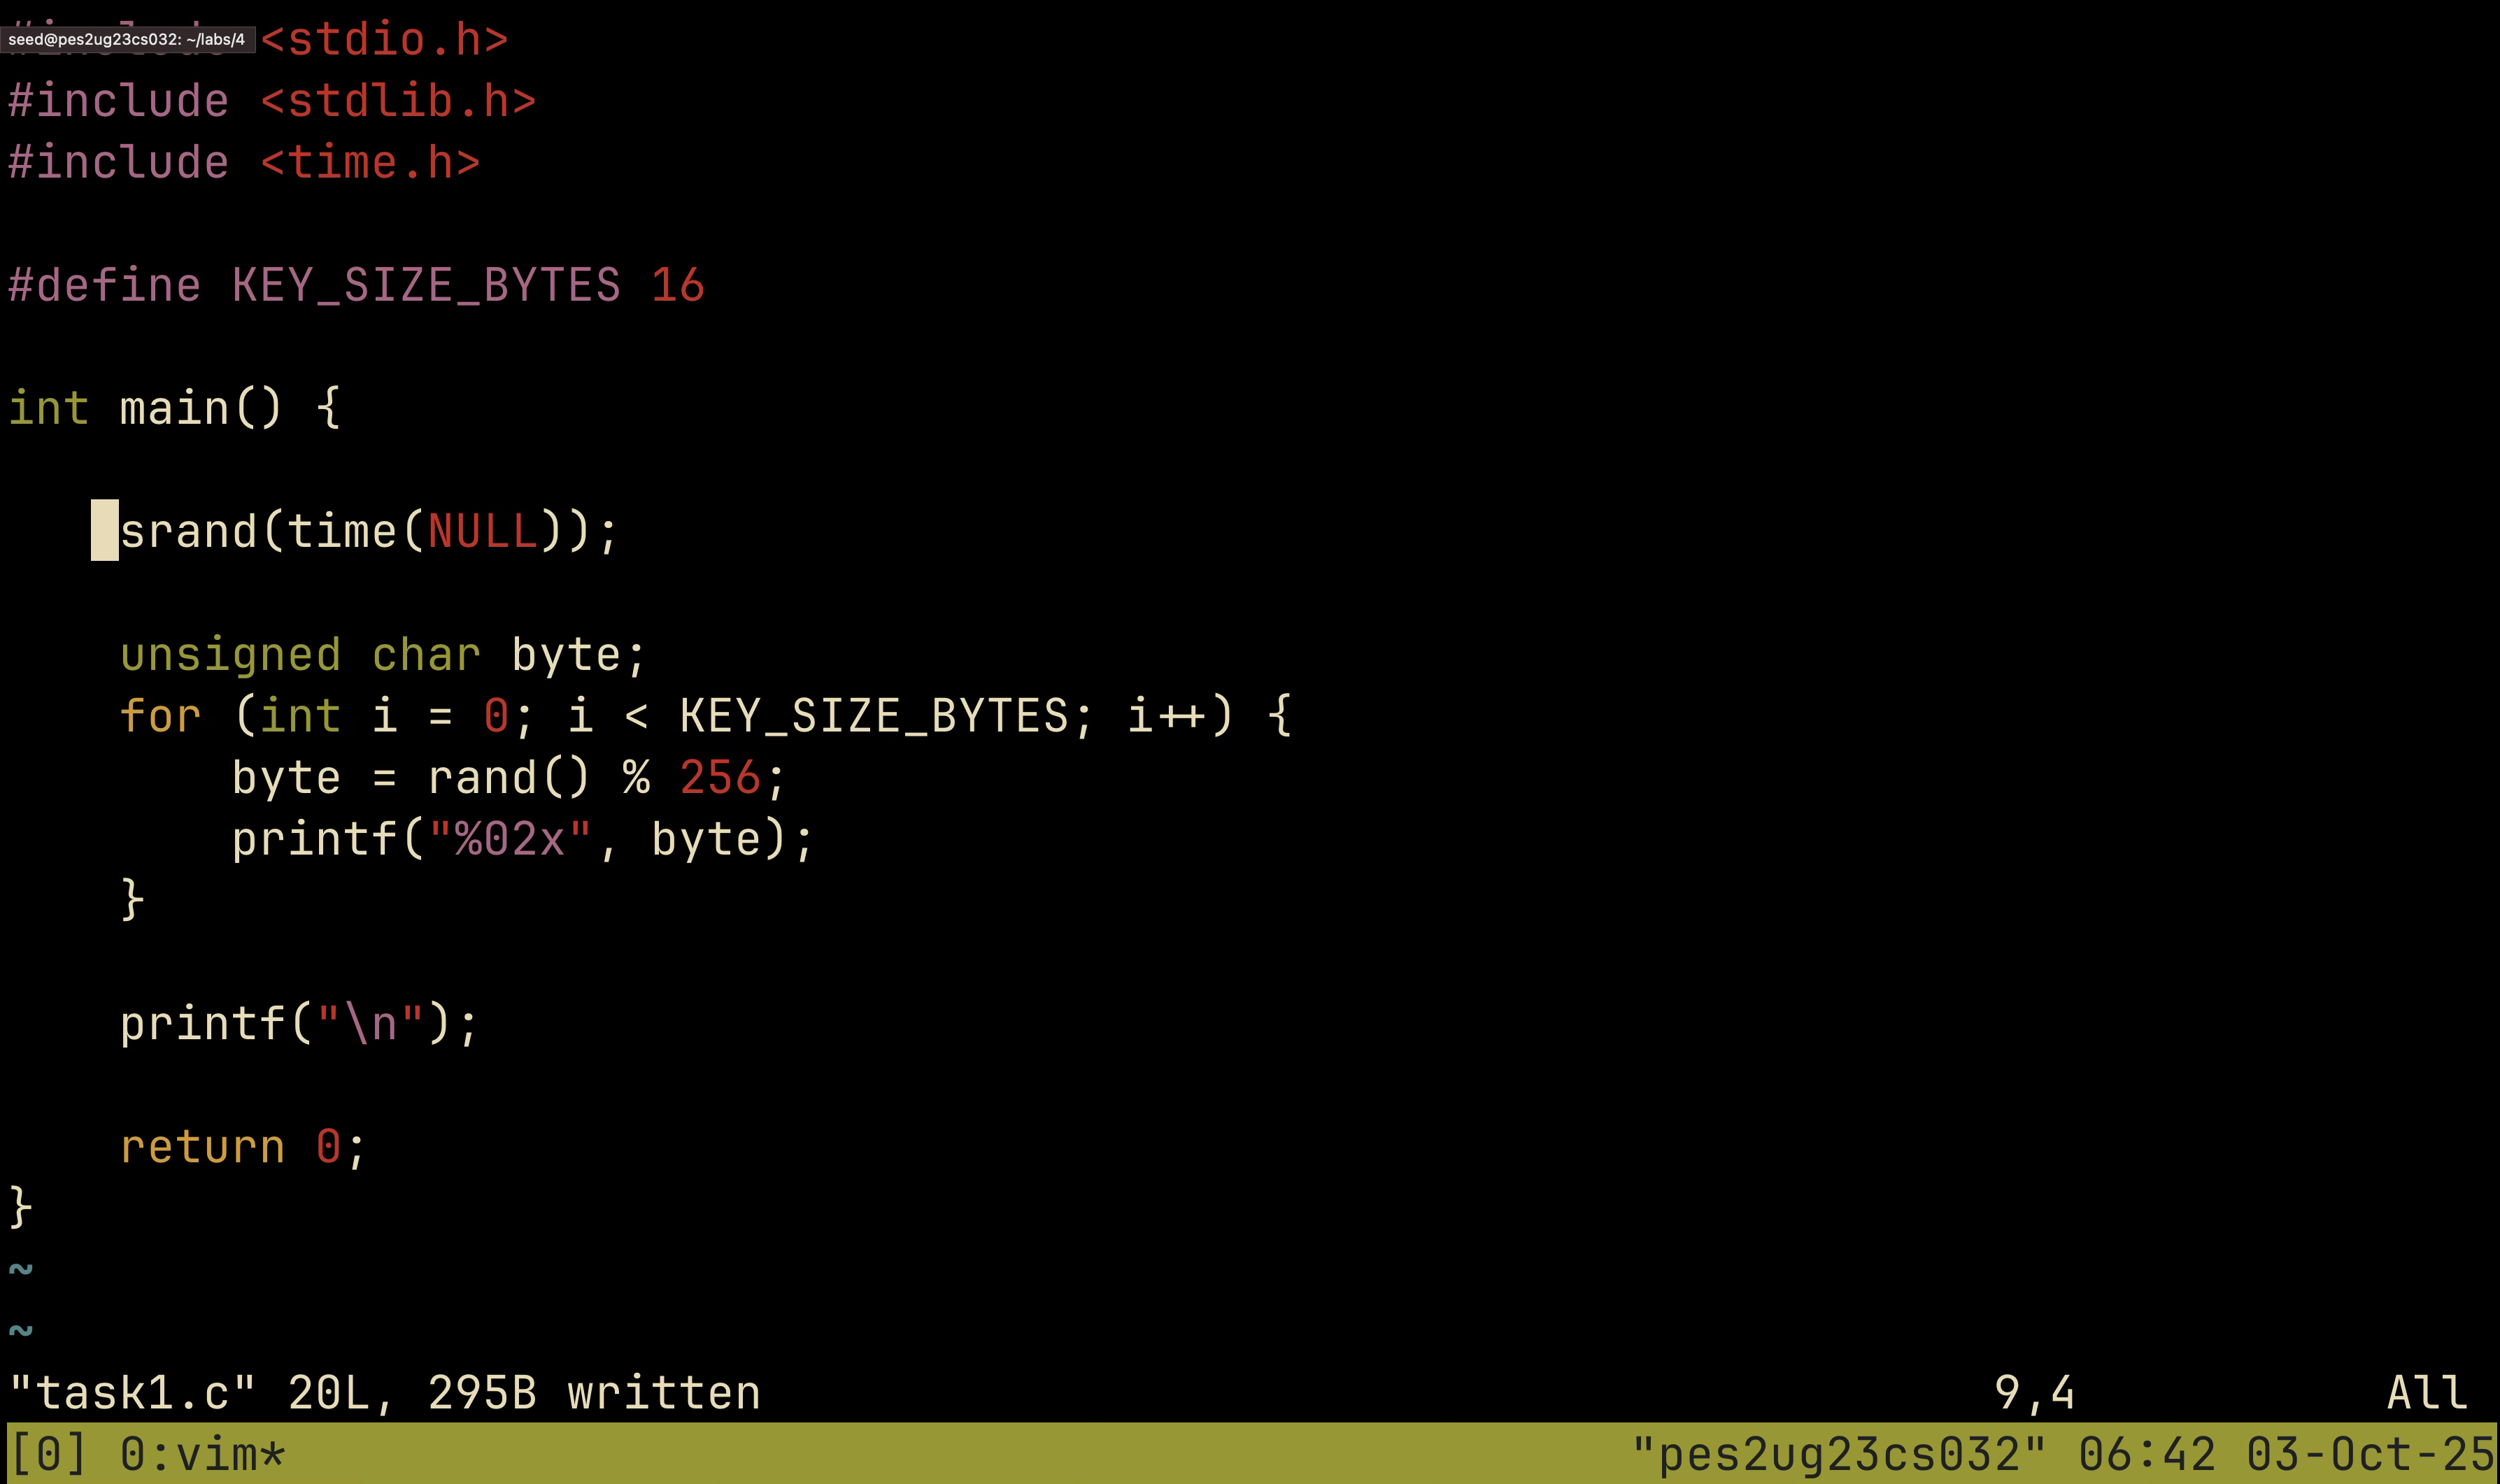
\includegraphics[width=0.8\textwidth]{./images/task1-1.png} 
\end{figure}

Running the program multiple times will yield a different key as the seed changes for each execution.

\begin{figure}[H]
    \centering
    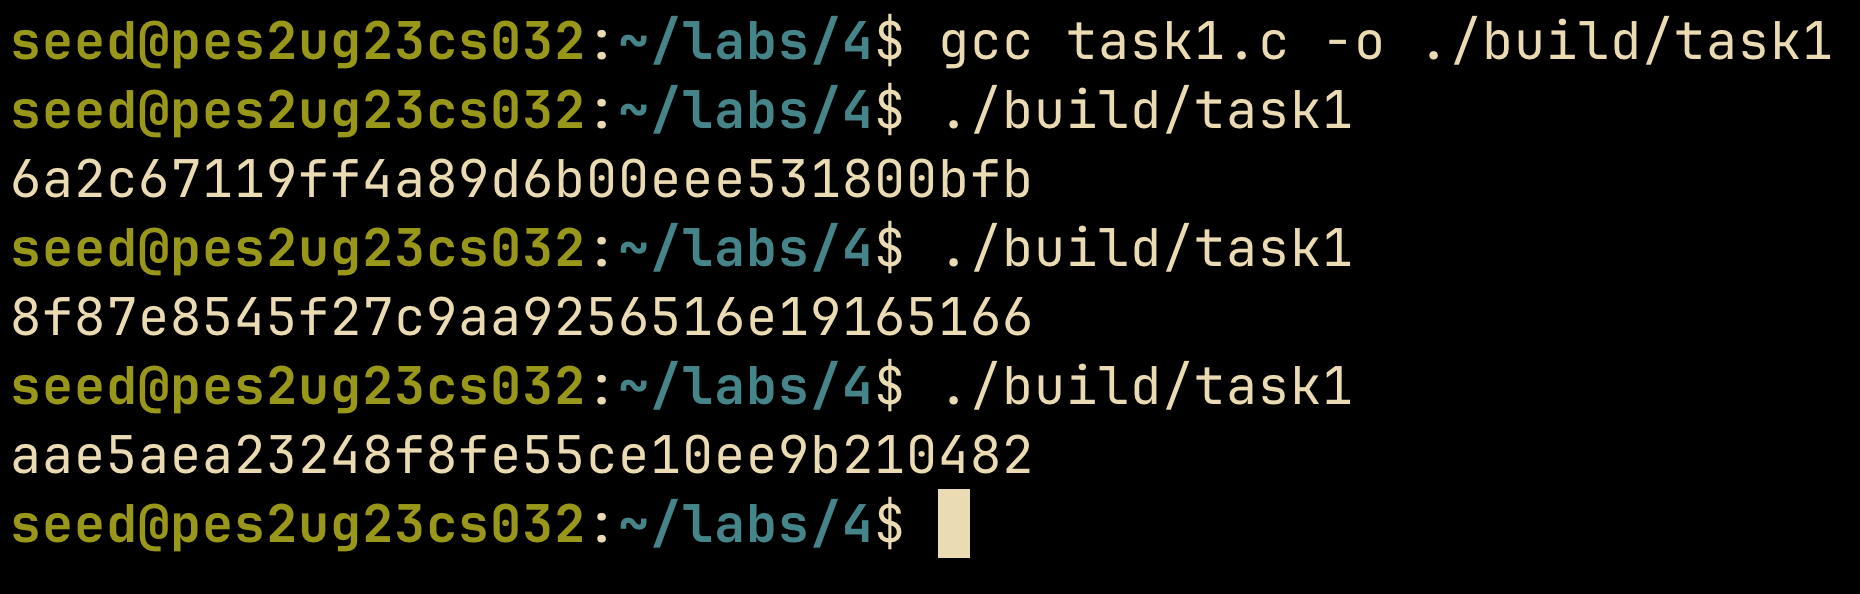
\includegraphics[width=0.8\textwidth]{./images/task1-2.png} 
\end{figure}

Removing the \texttt{srand()} will result in the program generating the same key for each execution. The seed for the compiled program will be the same regardless of when it is executed, hence being more deterministic.

\begin{figure}[H]
    \centering
    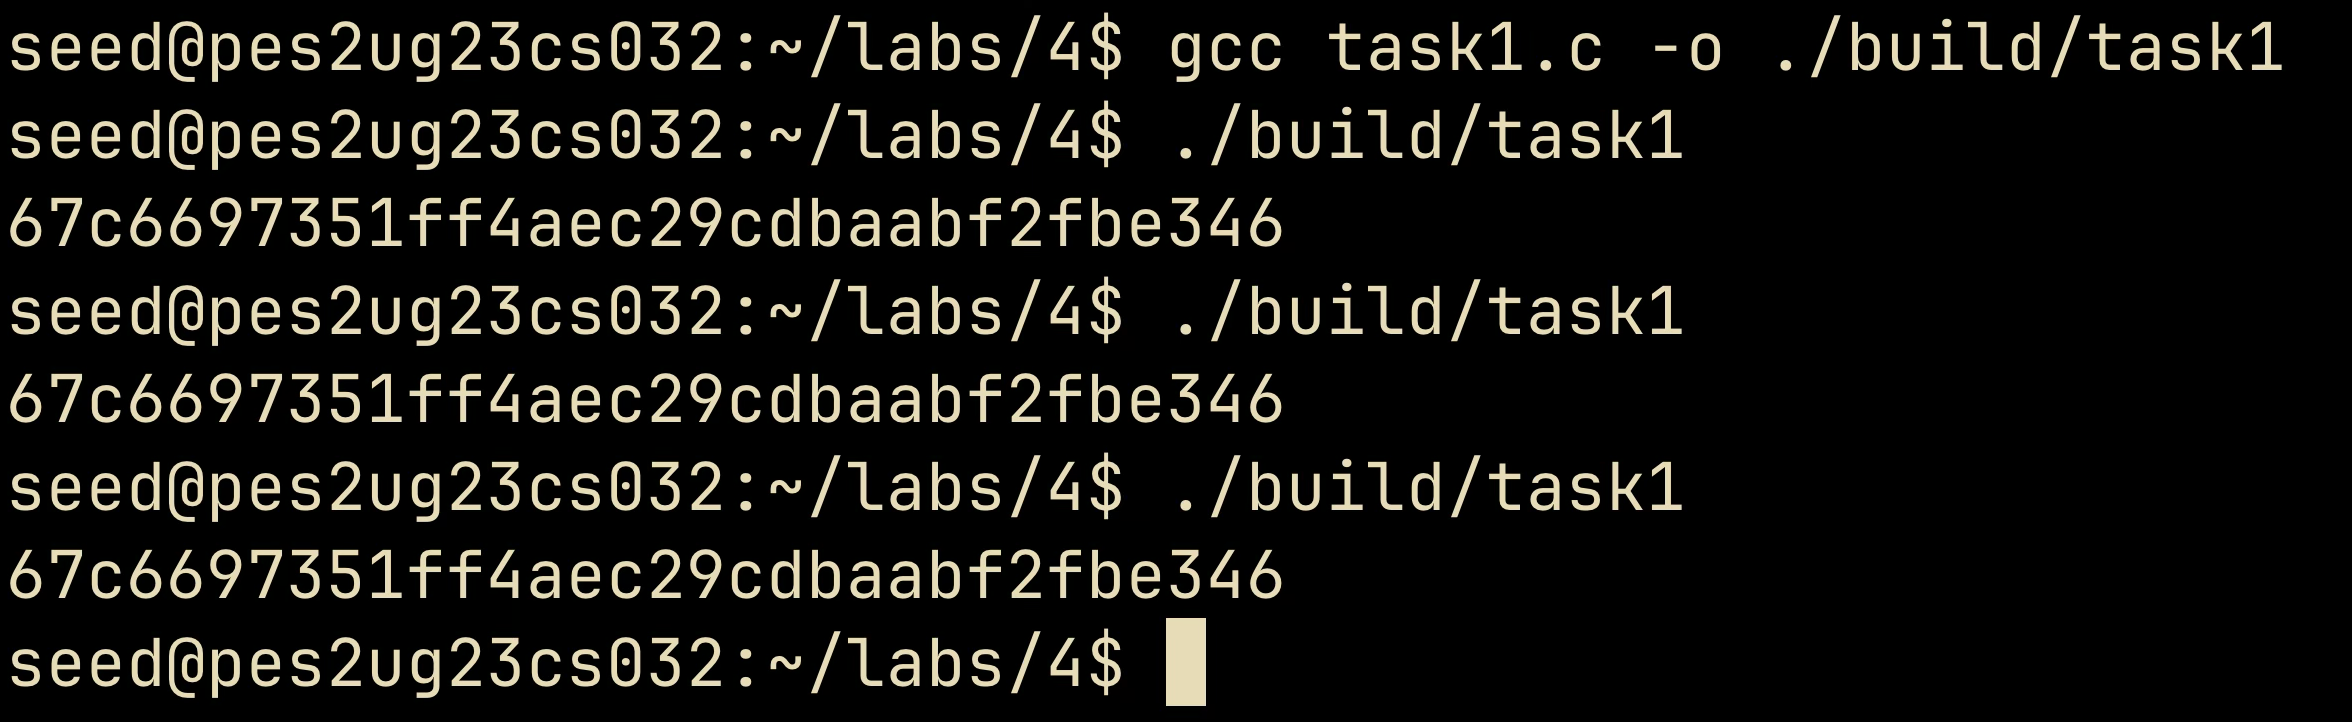
\includegraphics[width=0.8\textwidth]{./images/task1-3.png} 
\end{figure}

\section{Task 2: Guessing the Key (Brute Force)}

Given to us is a time stamp range \texttt{2018\@-04\@-17 21:08:49} to \texttt{2018\@-04\@-17 23:08:49} during which a key was generated. We are also given the following:

\begin{enumerate}
    \item cipher text \texttt{d06bf9d0dab8e8ef880660d2af65aa82}
    \item plaintext \texttt{255044462d312e350a25d0d4c5d80a34}
\end{enumerate}

First we convert the given timestamp to the UNIX epoch. From trial and error, the epoch for the start time is taken with the timezone \texttt{Etc/GMT+4}.

\begin{figure}[H]
    \centering
    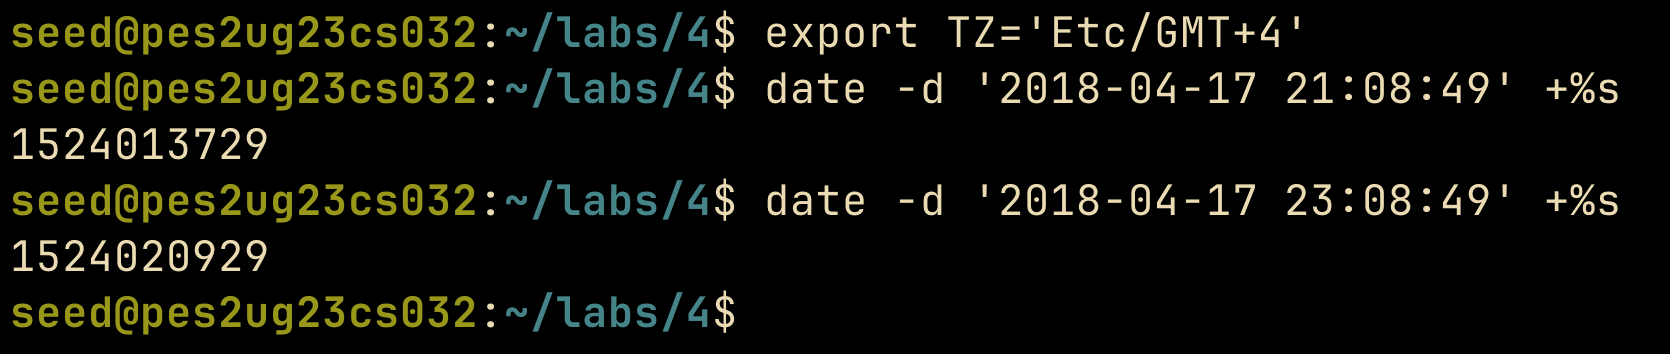
\includegraphics[width=0.8\textwidth]{./images/task2-1.png} 
\end{figure}

Using the given range of timestamps, we generate all the keys possible and store it in a file named \texttt{keys.txt}.

\begin{figure}[H]
    \centering
    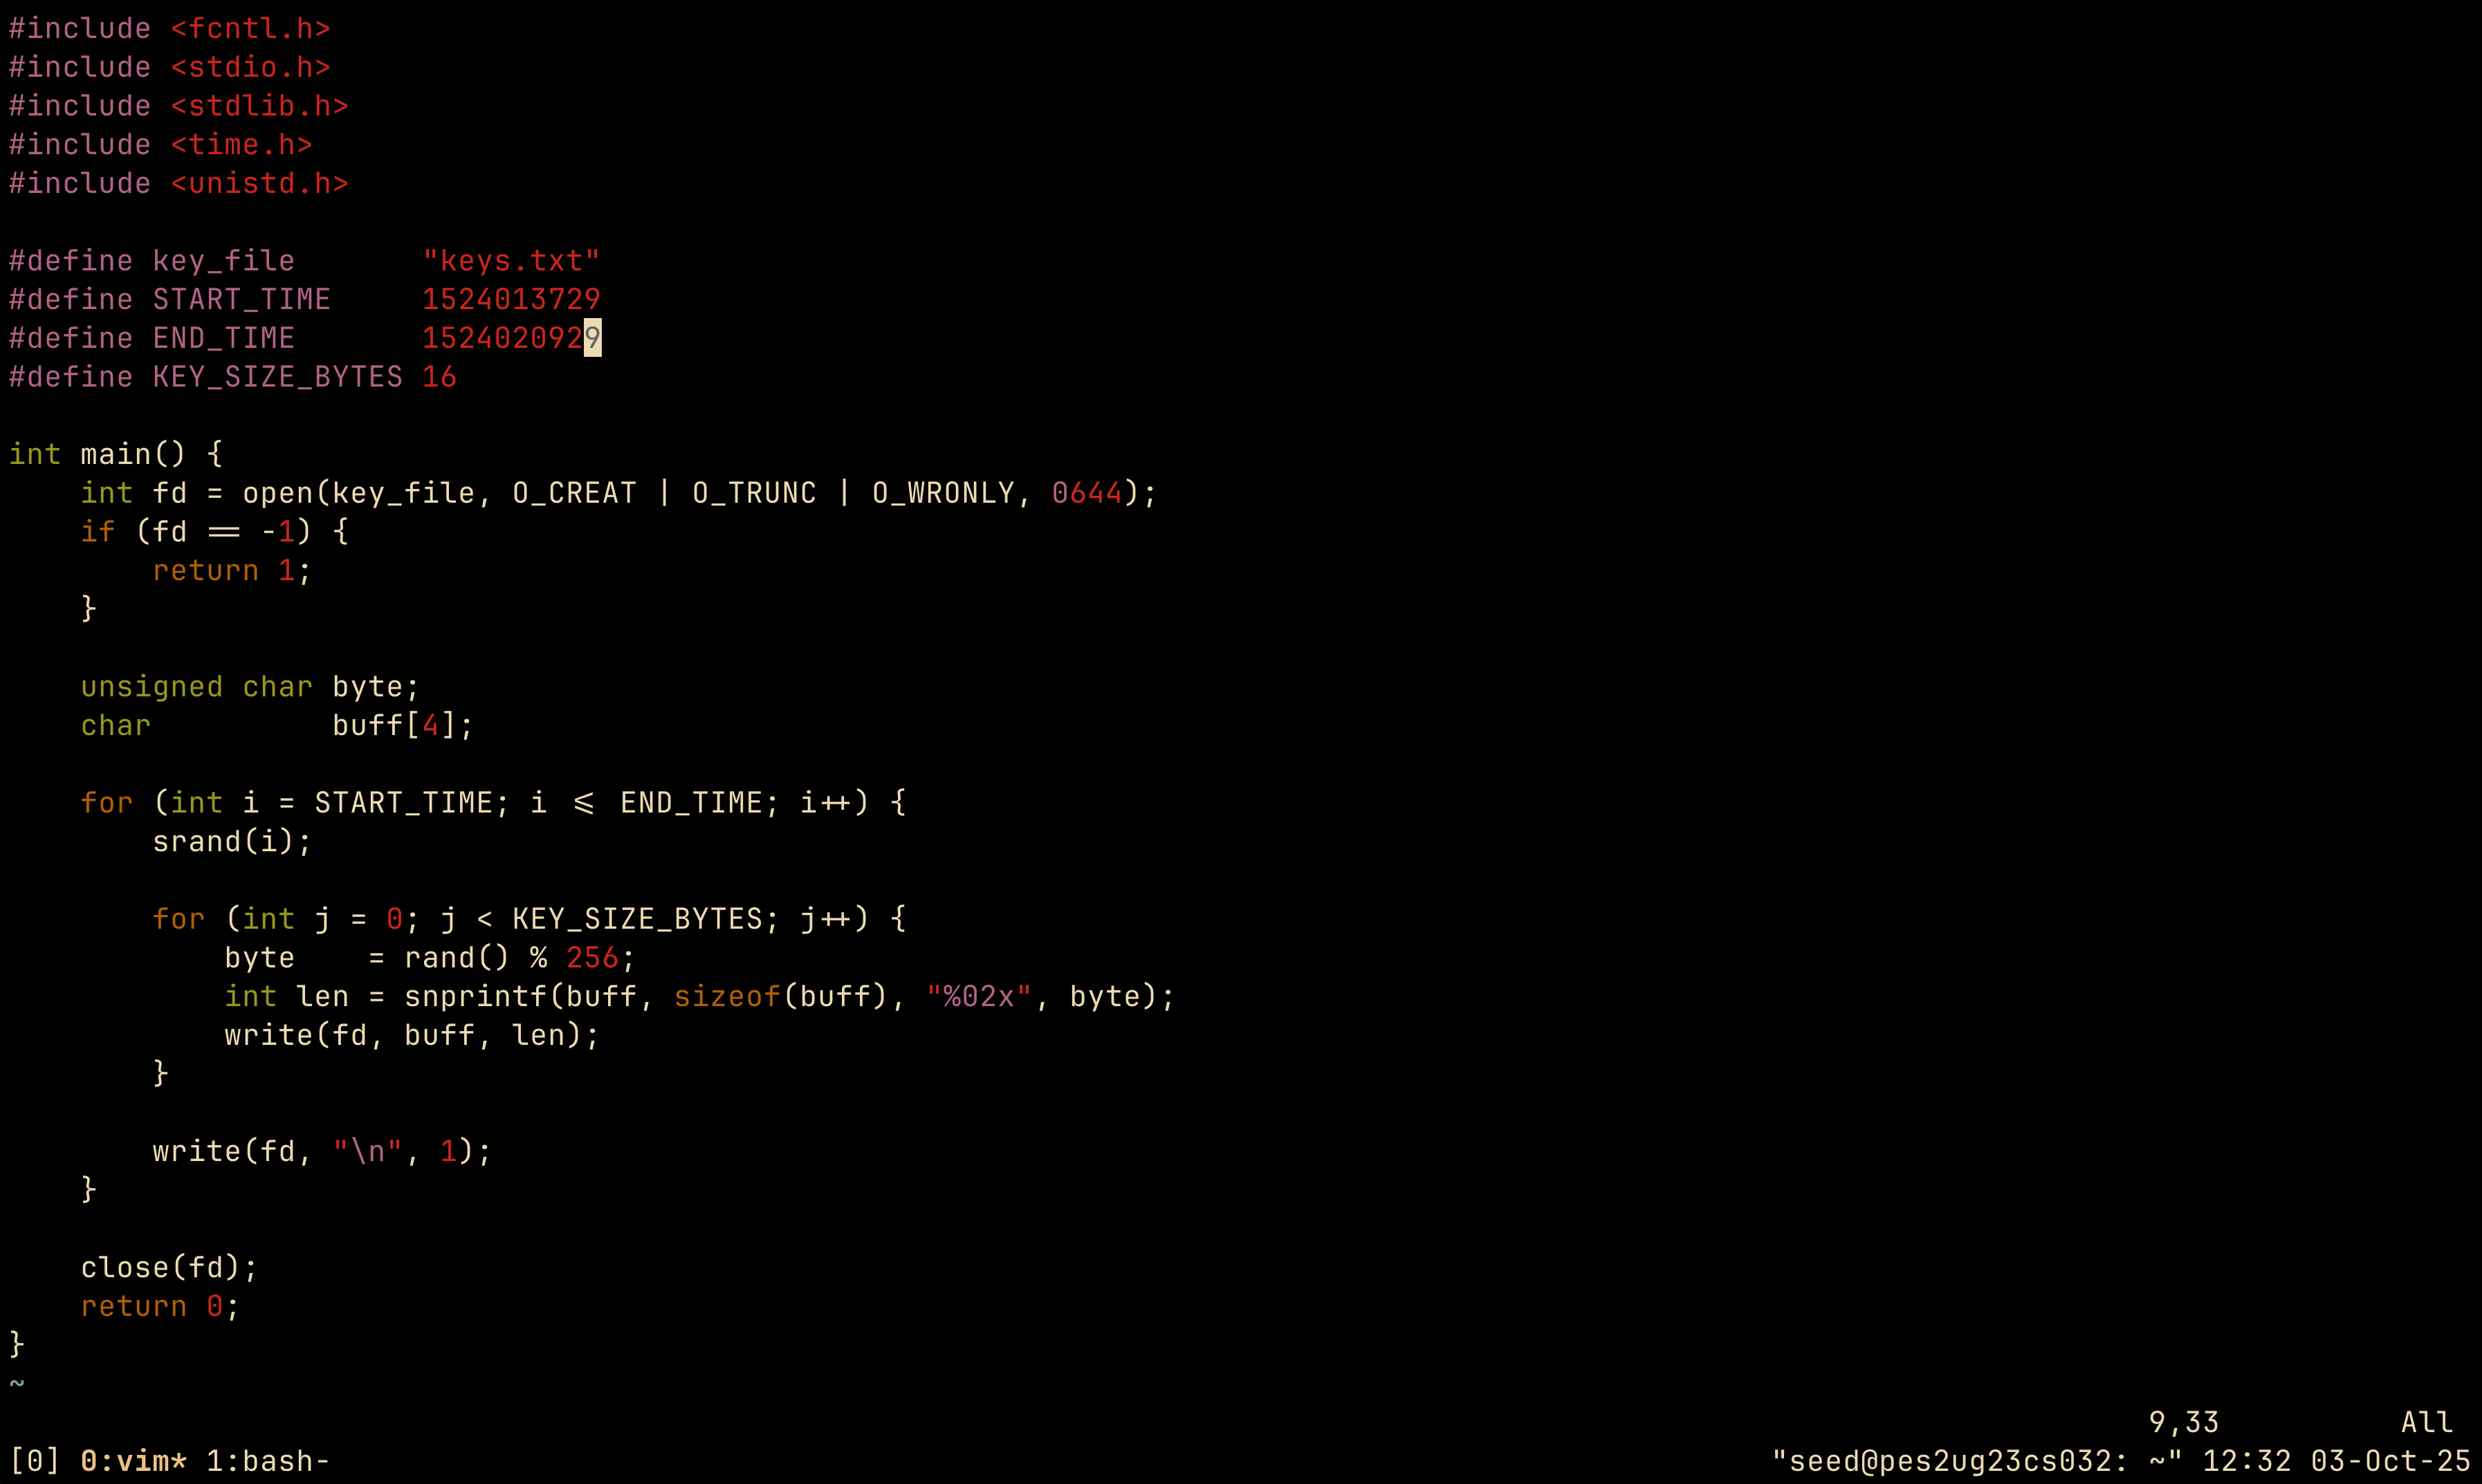
\includegraphics[width=0.8\textwidth]{./images/task2-2.png} 
\end{figure}

\begin{figure}[H]
    \centering
    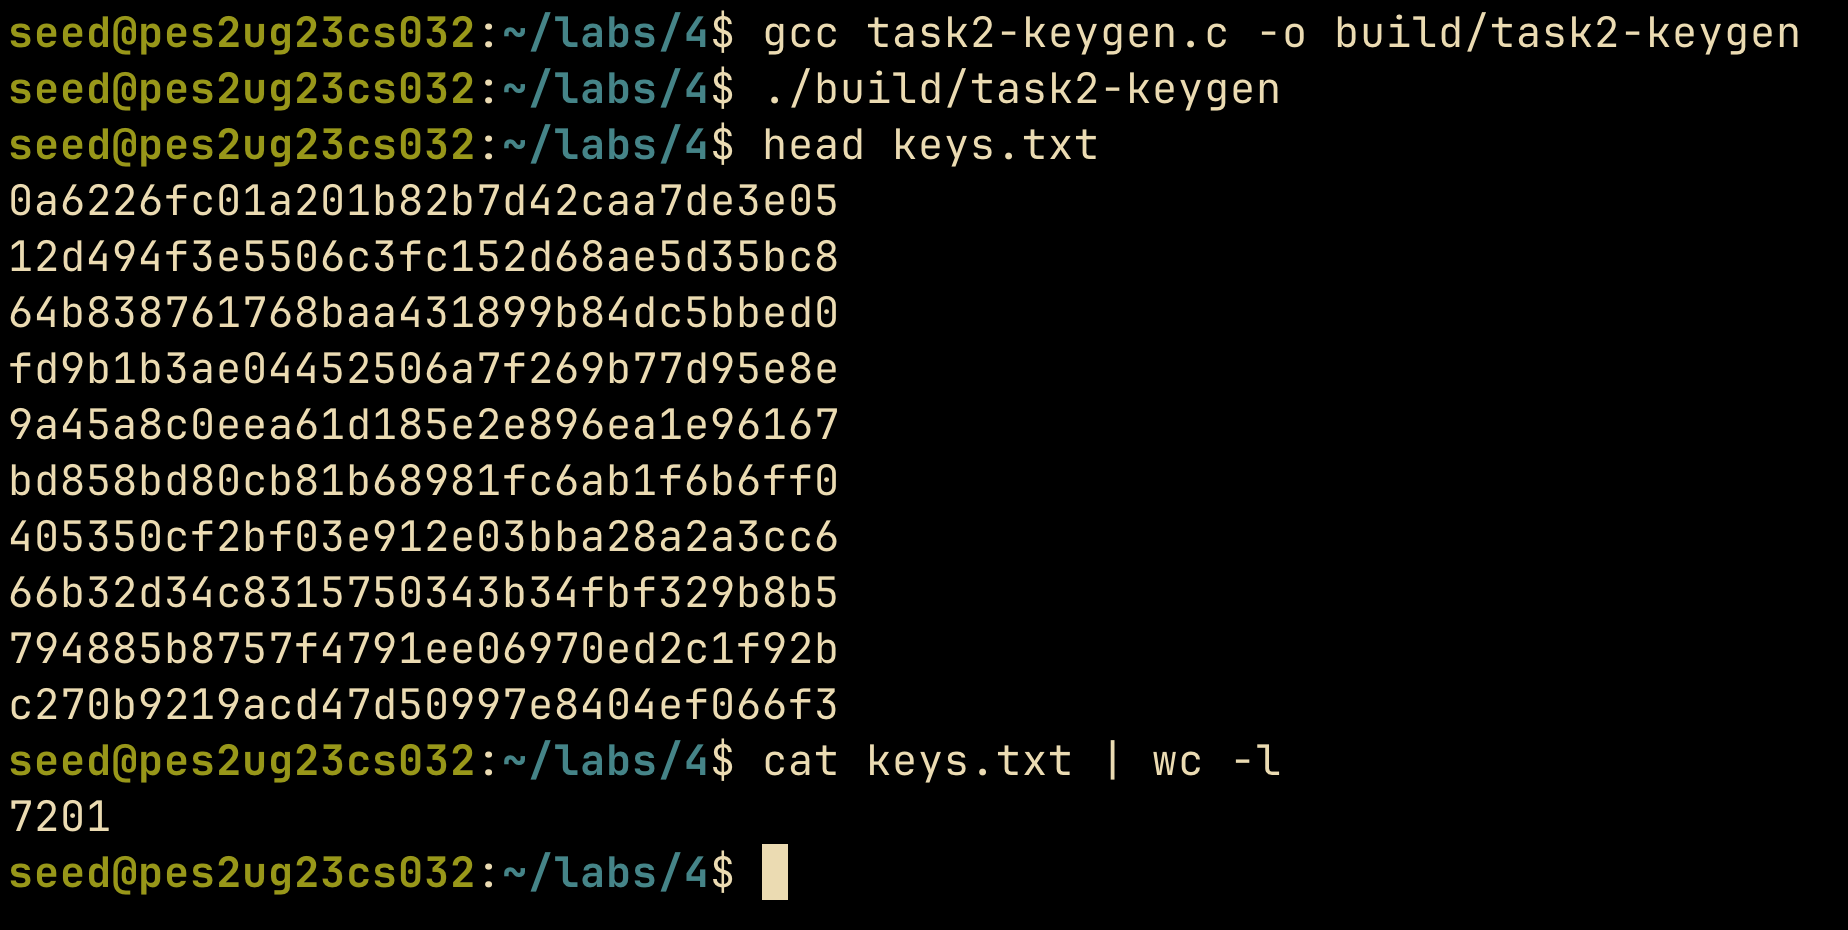
\includegraphics[width=0.8\textwidth]{./images/task2-3.png} 
\end{figure}

Now with the following python code, we iterate over every key in the file and generate the cipher text for the given plain text with AES-128-CBC mode and return the ciphertext and key that matches with the given cipher text.

\begin{figure}[H]
    \centering
    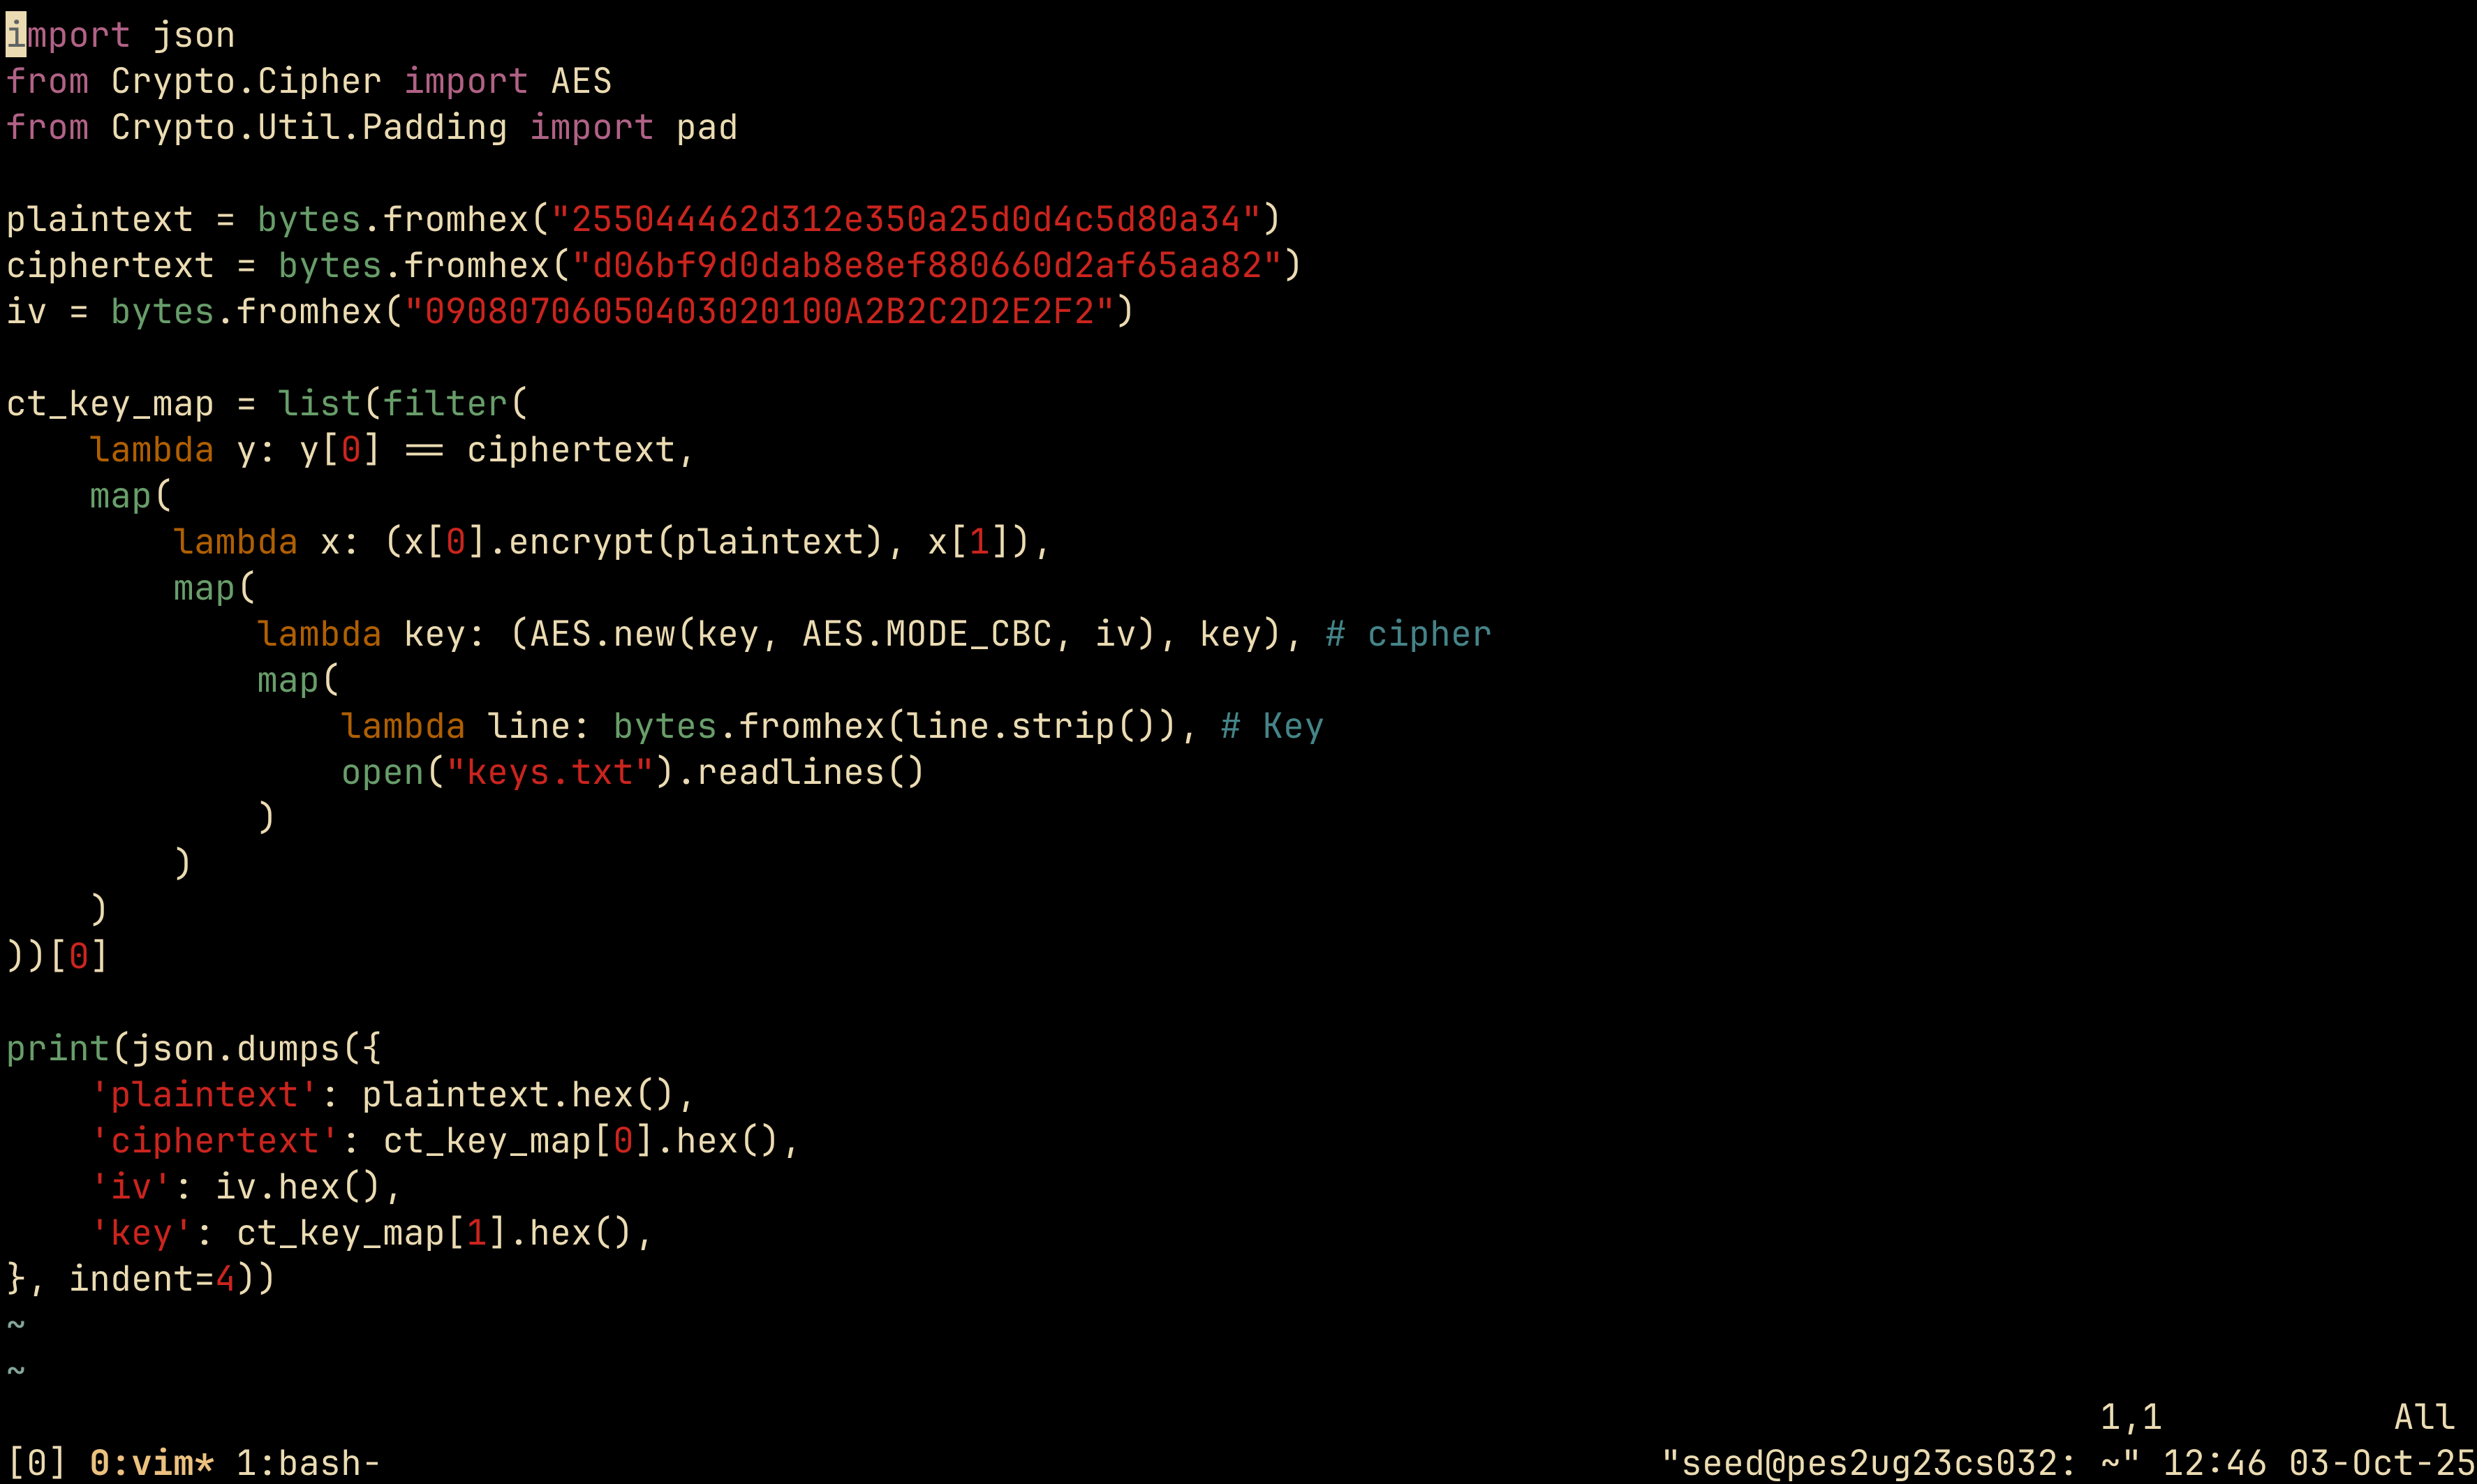
\includegraphics[width=0.8\textwidth]{./images/task2-4.png} 
\end{figure}

\begin{figure}[H]
    \centering
    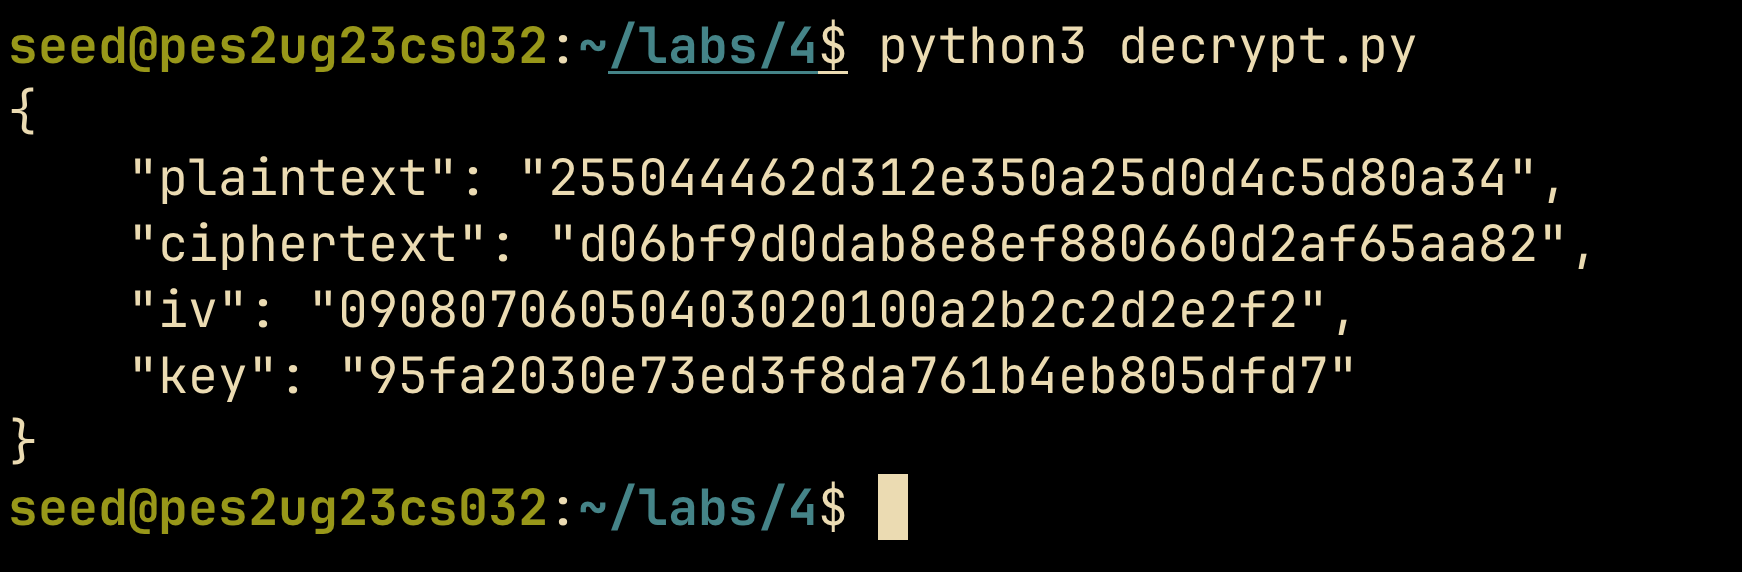
\includegraphics[width=0.8\textwidth]{./images/task2-5.png} 
\end{figure}

\pagebreak

\section{Task 3: Measuring Kernel Entropy}

\begin{figure}[H]
    \centering
    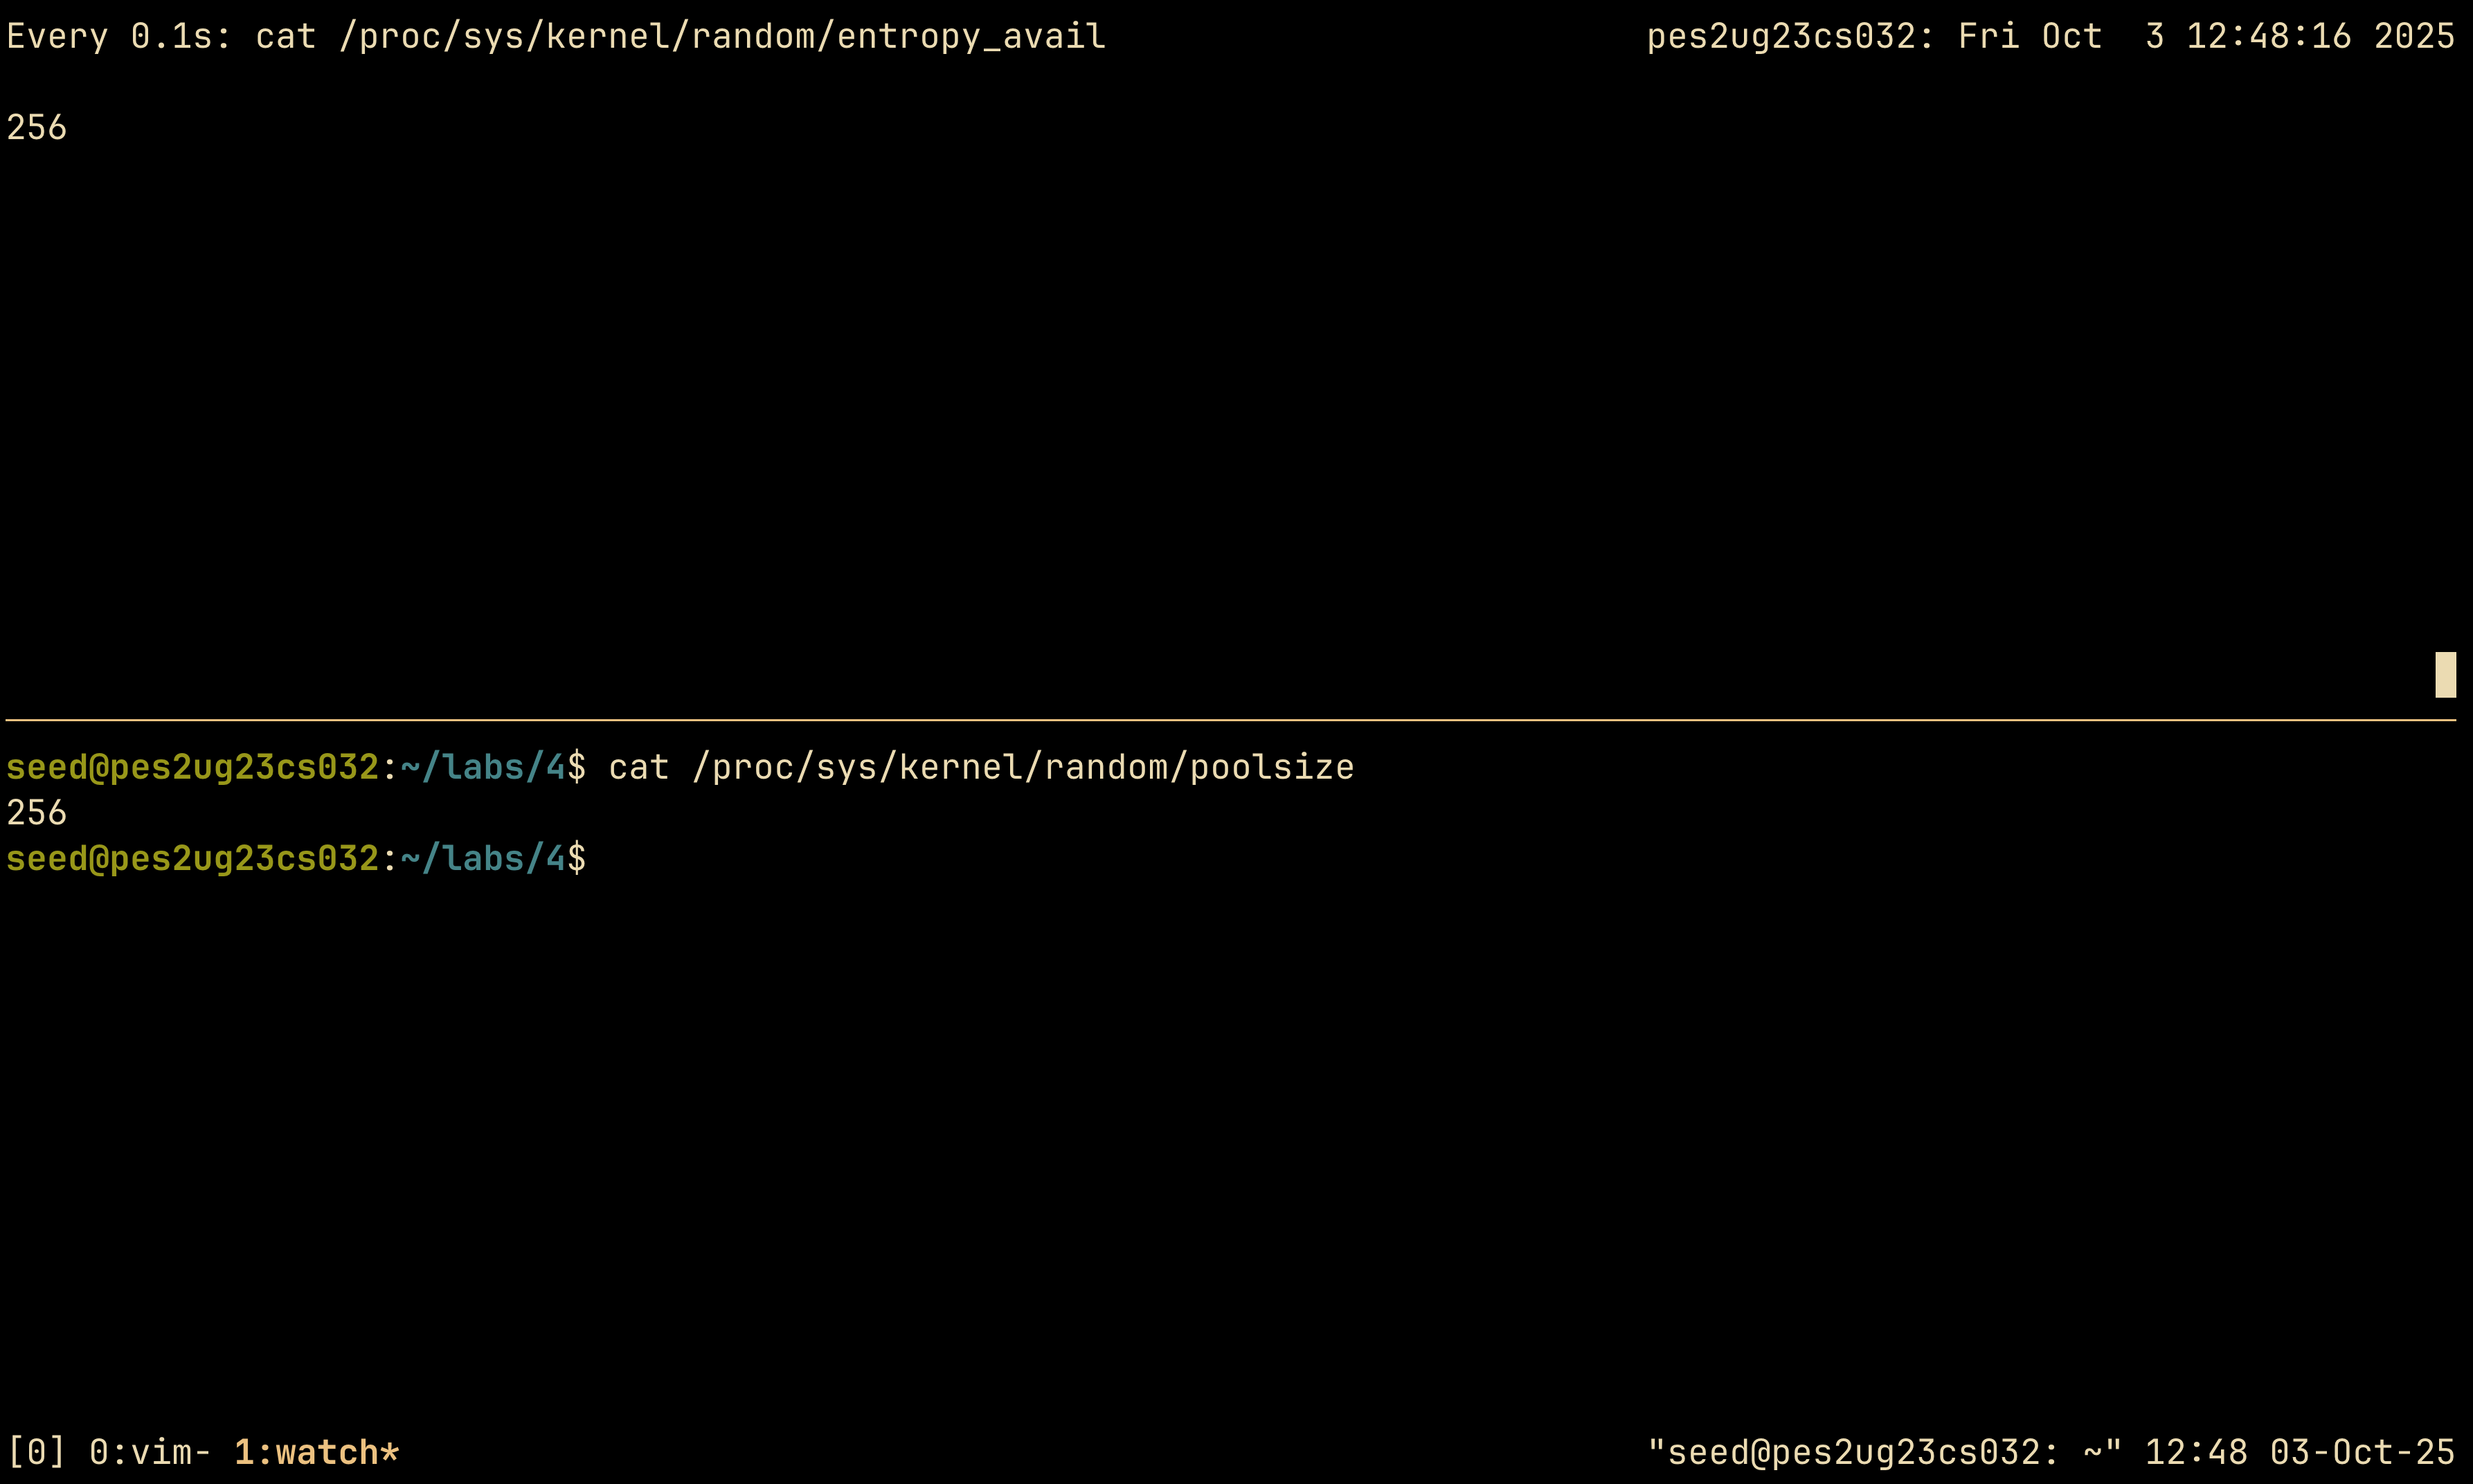
\includegraphics[width=0.8\textwidth]{./images/task3.png} 
\end{figure}

The expected outcome is the entropy value will change over time as the entropy pool is filled as the system collects randomness for various sources. However, in this case the entropy pool is fixed at 256 bits. The system is currently using the linux 5.15.0-152-generic kernel. After a commit to the linux kernel \url{https://git.kernel.org/pub/scm/linux/kernel/git/stable/linux.git/log/?h=linux-5.15.y&ofs=3200}, the entropy pool size has been changed from $\approx$4096 bits to 256 bits. There has also been a change in the way the entropy is calculated as well. Hence simulating a change in the value in \texttt{entrop\_avail} is not possible in this report.

\section{Task 4: Generating PSRNG from \texttt{/dev/random}}

\begin{figure}[H]
    \centering
    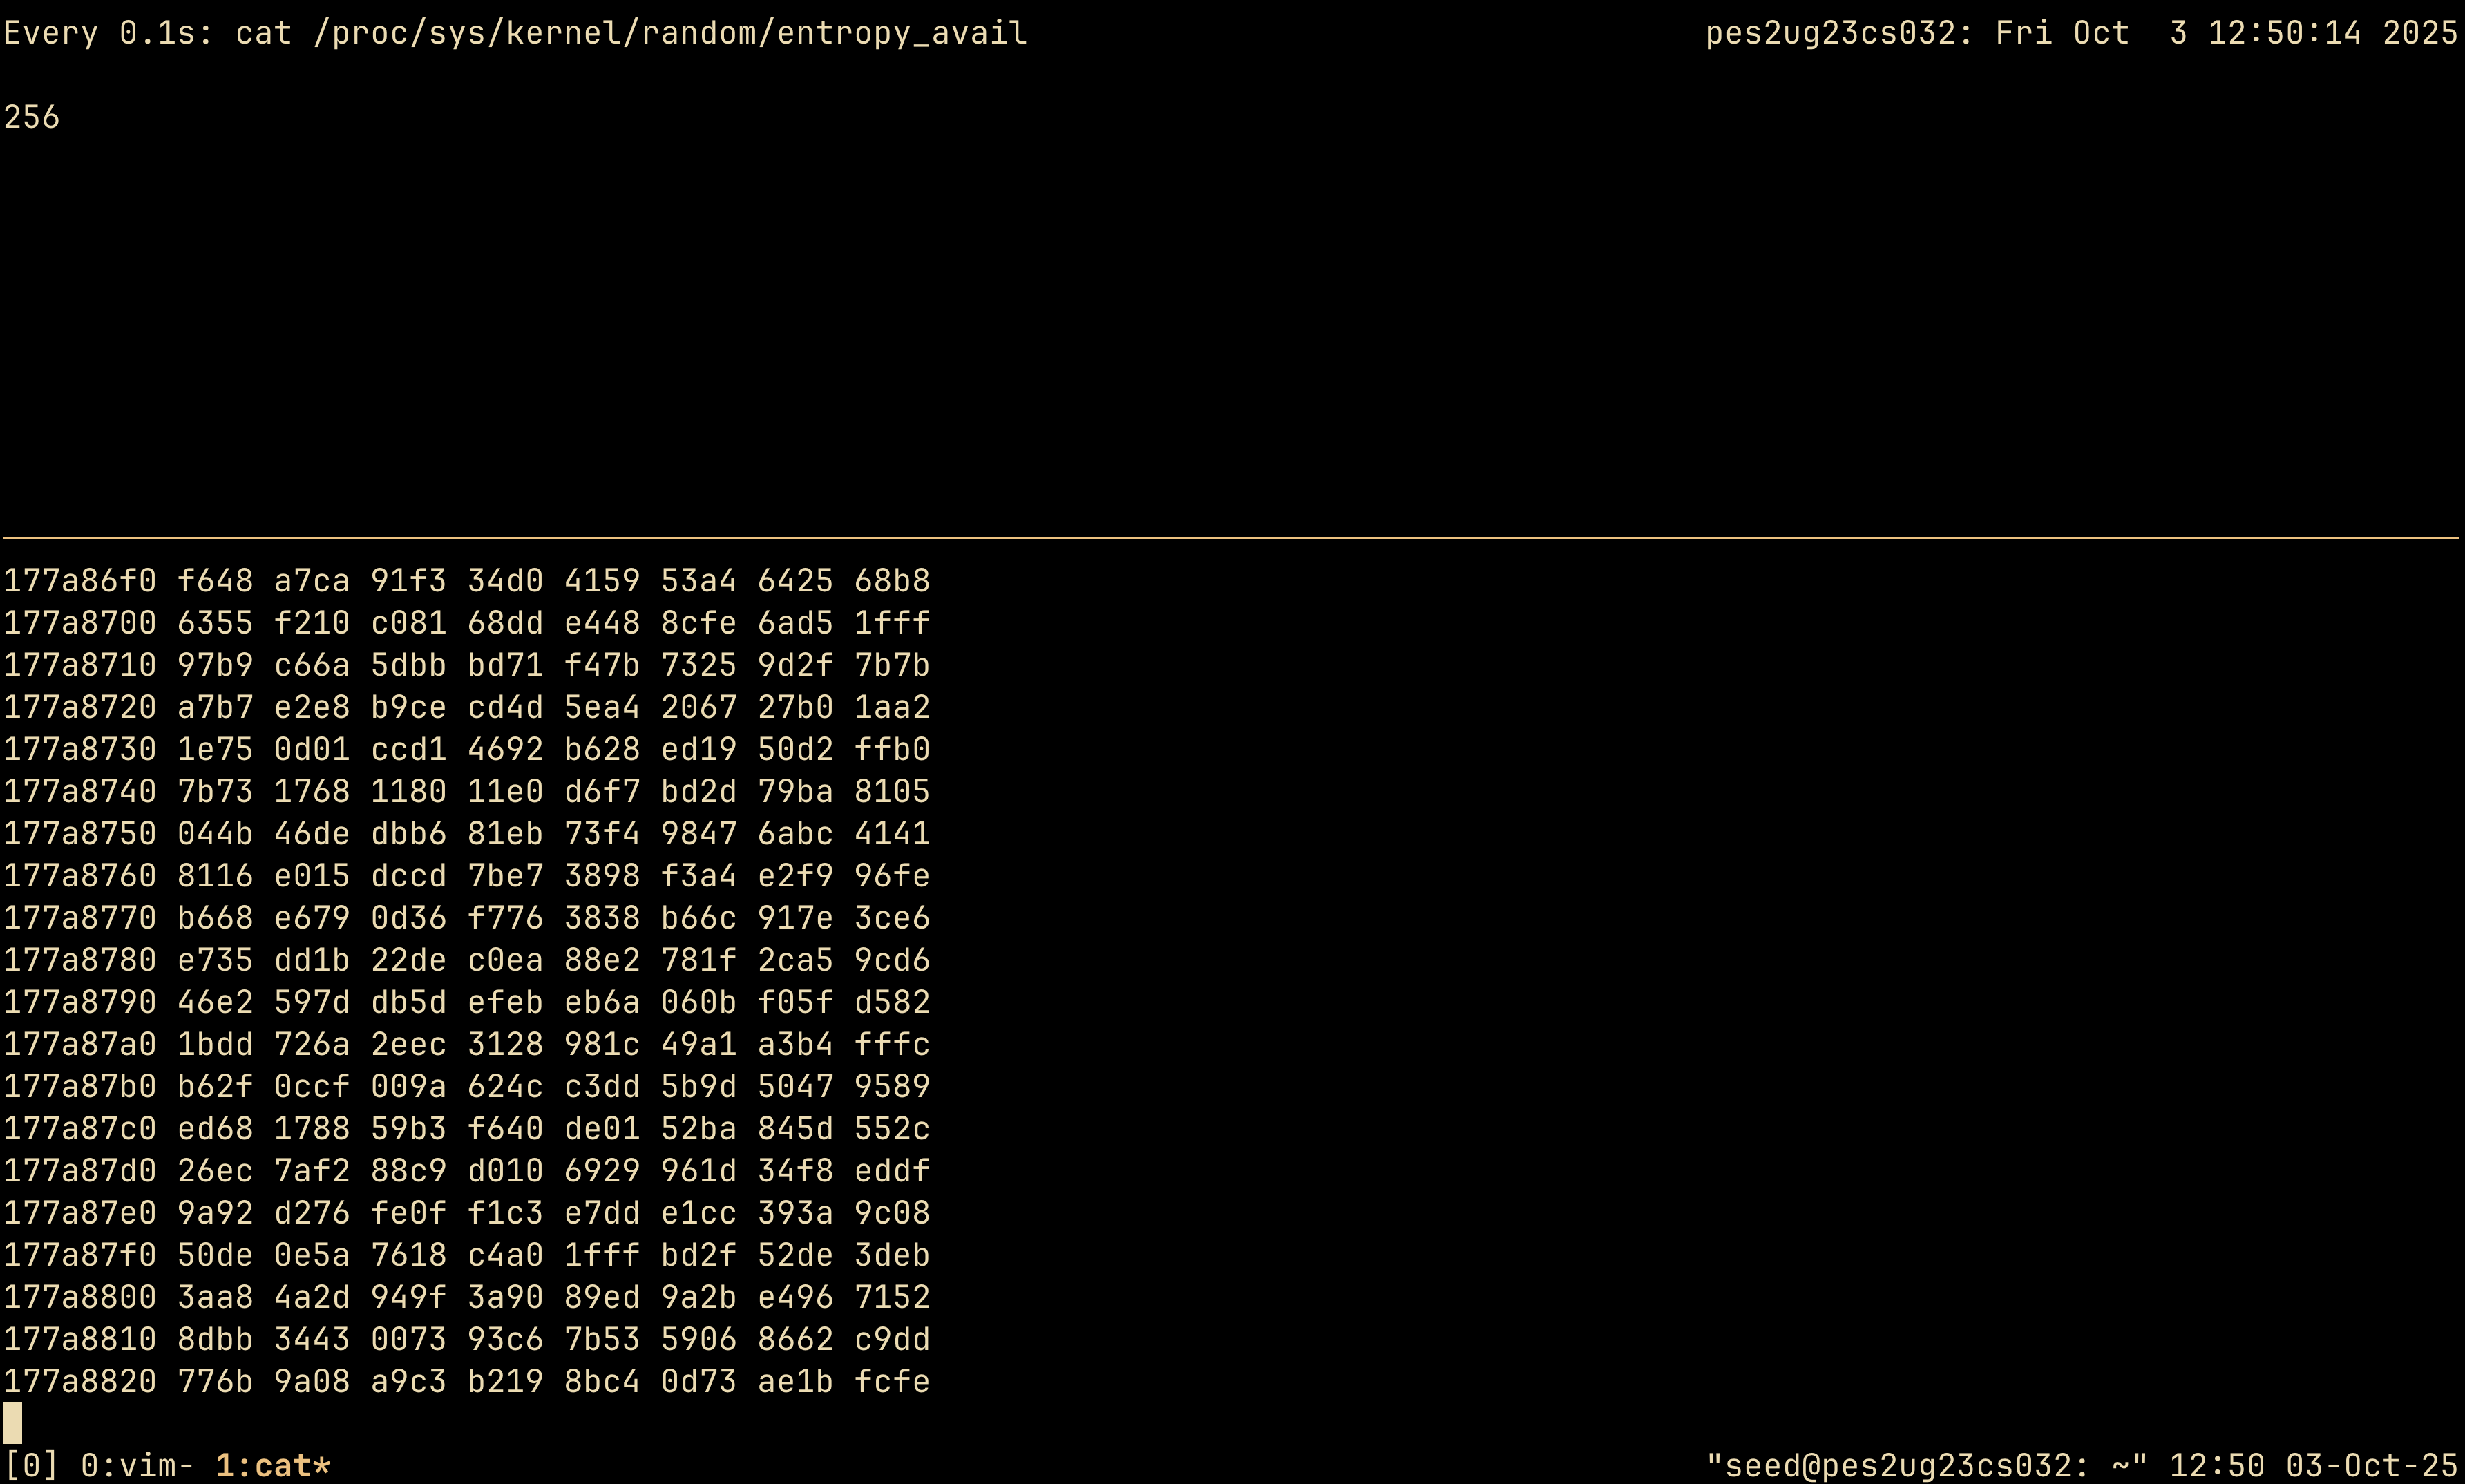
\includegraphics[width=0.8\textwidth]{./images/task4.png} 
\end{figure}

\section{Task 5: Measuring Entropy of \texttt{/dev/urandom}}

\begin{figure}[H]
    \centering
    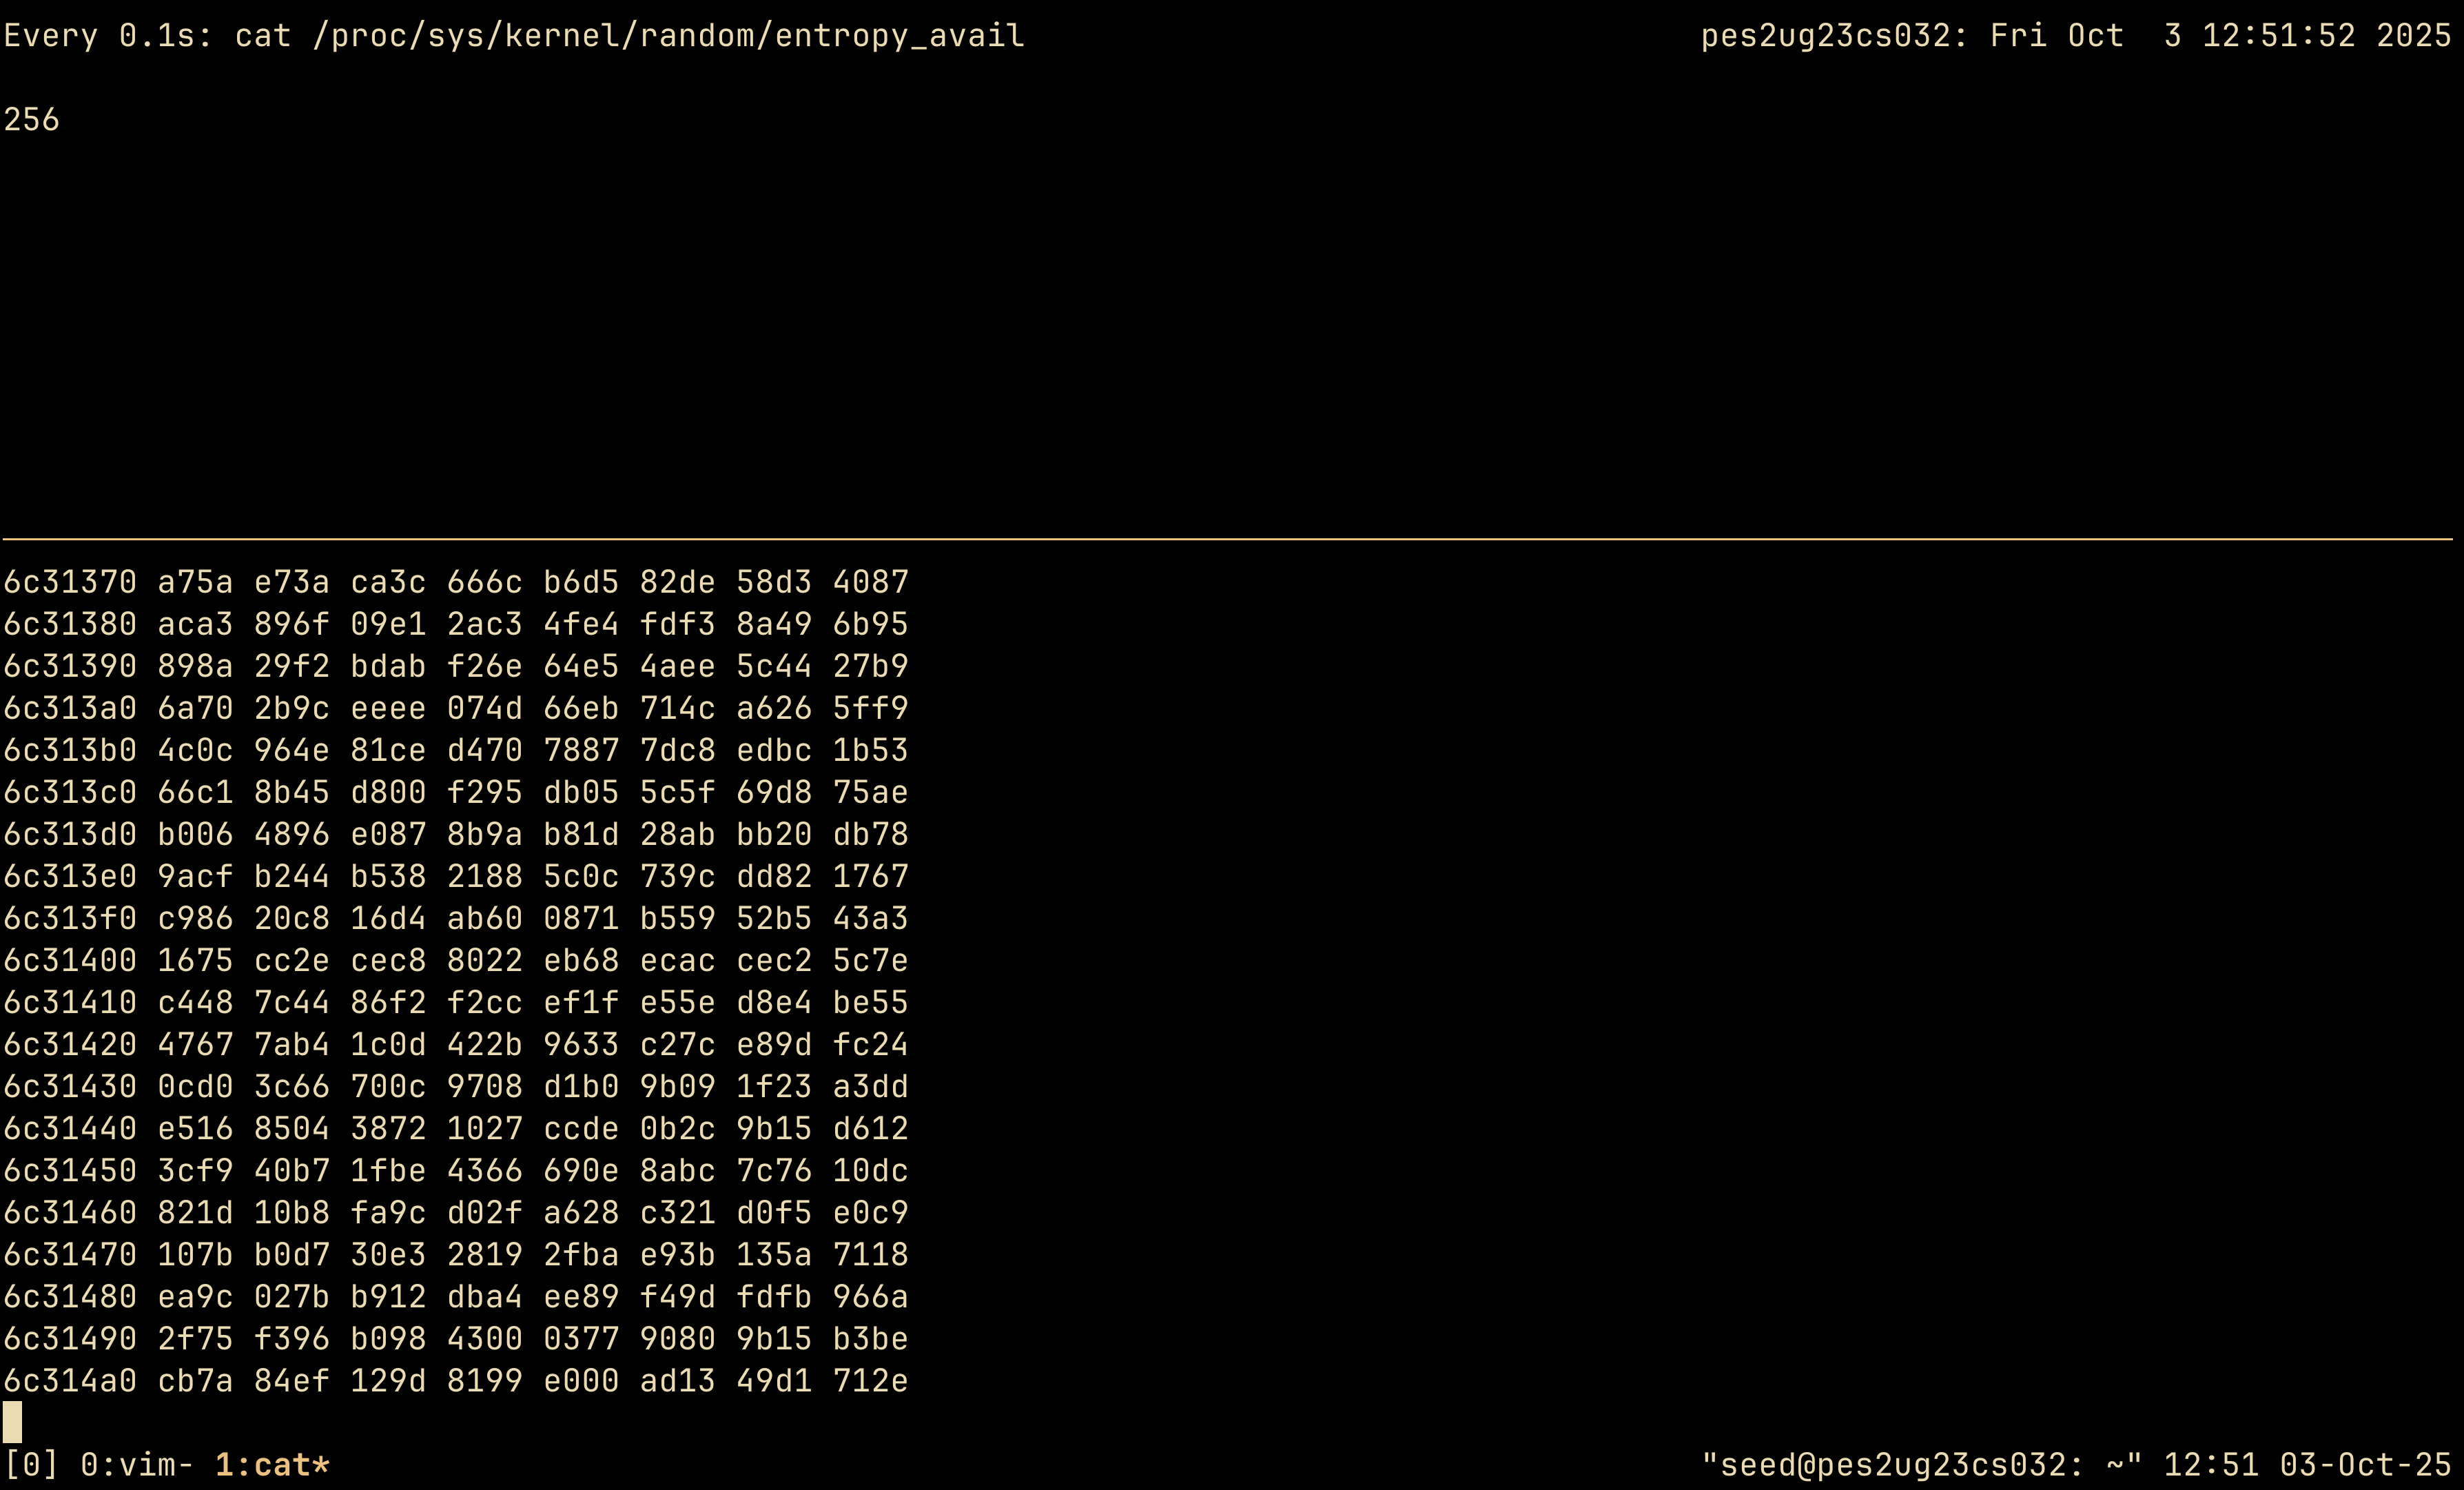
\includegraphics[width=0.8\textwidth]{./images/task5-1.png} 
\end{figure}

\begin{figure}[H]
    \centering
    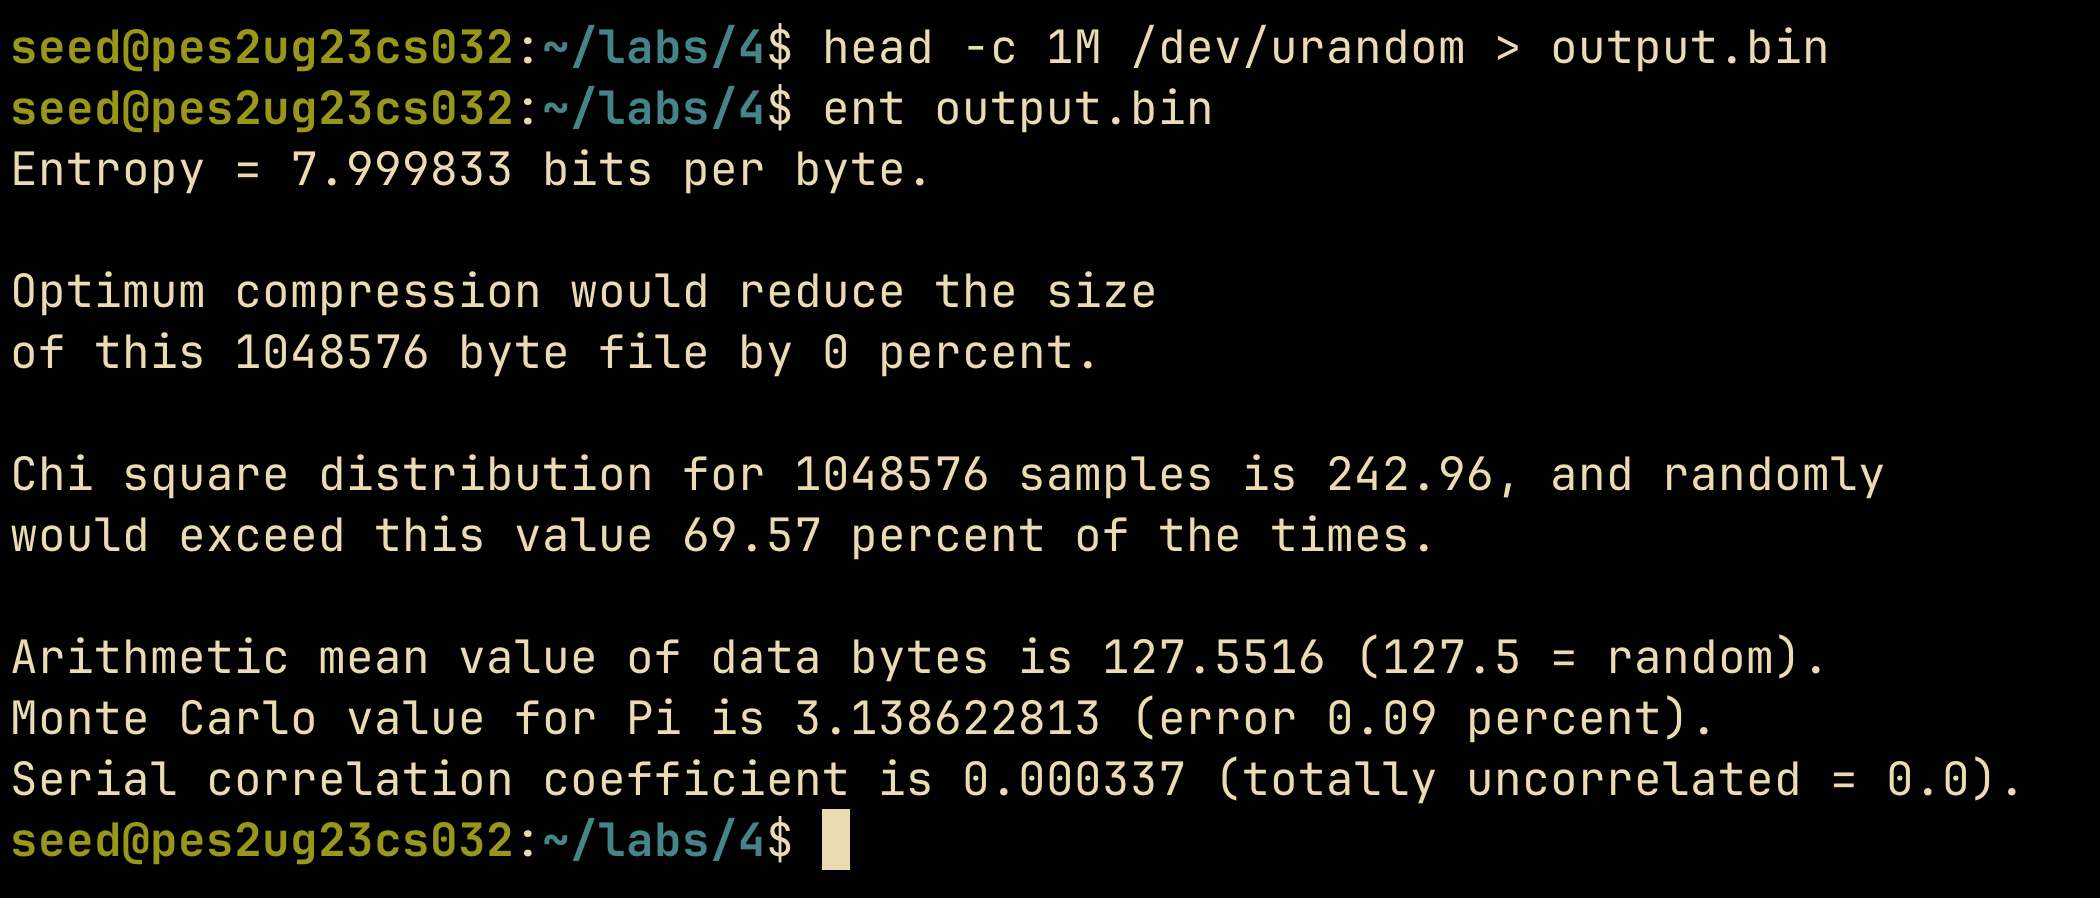
\includegraphics[width=0.8\textwidth]{./images/task5-2.png} 
\end{figure}

from the ent output, we can conclude that

\begin{enumerate}
    \item Entropy at 7.999833 bits per byte, close to the ideal value of 8 makes it suitable for cryptographic applications, it is highly random.
    \item The chi square value 242.98 is within the expected range of randomness, tests if the distribution is uniform.
    \item Monte Carlo value for Pi has an error of 0.093\%, uses randomness to estimate the value of Pi.
    \item Serial correlation coefficient is close to 0, there are no patterns hence its highly random.
\end{enumerate}

\pagebreak

\section{Task 6: Encryption using Different Ciphers and Modes}

\begin{figure}[H]
    \centering
    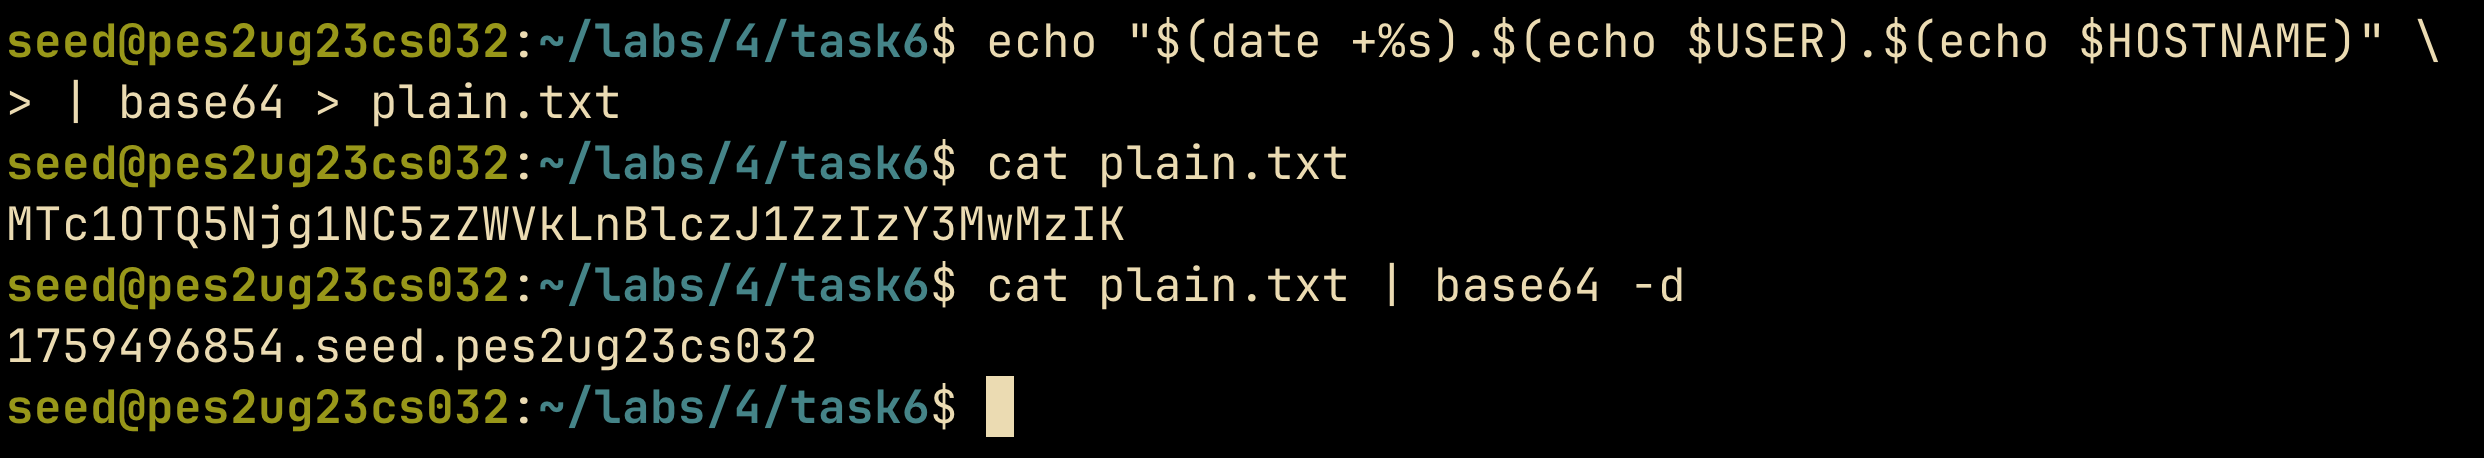
\includegraphics[width=0.8\textwidth]{./images/task6-1.png} 
    \caption{Generating the plaintext}
\end{figure}

\begin{figure}[H]
    \centering
    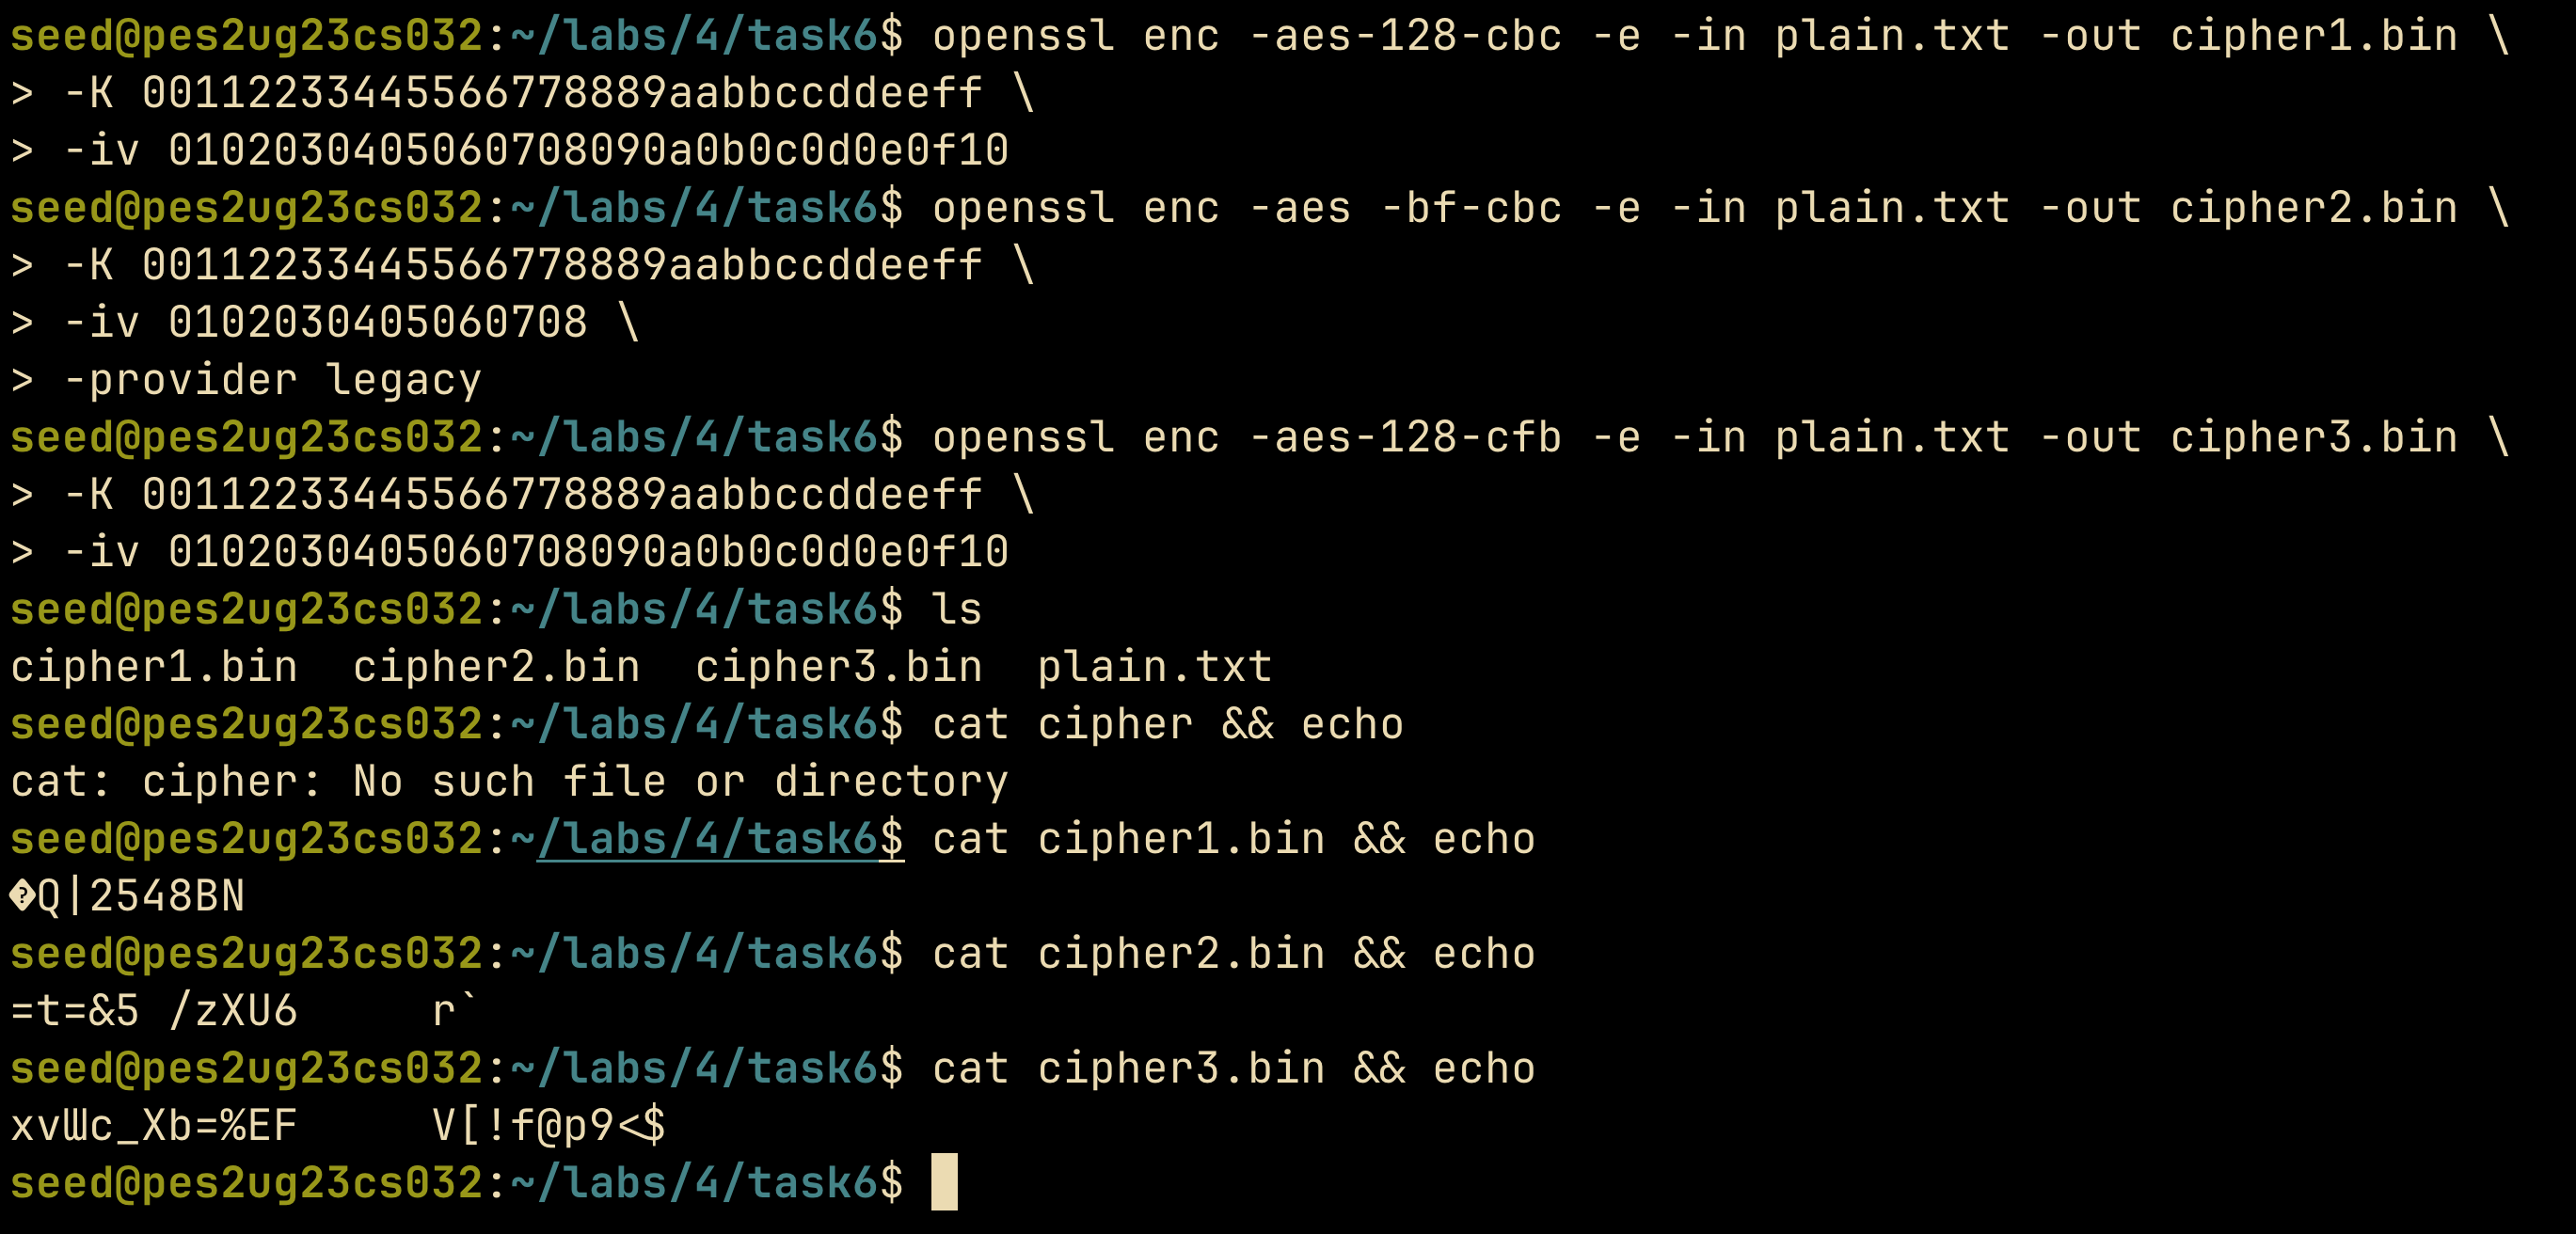
\includegraphics[width=0.8\textwidth]{./images/task6-2.png} 
    \caption{Encrypting with \texttt{openssl} with different modes of AES and Blowfish}
\end{figure}

\begin{figure}[H]
    \centering
    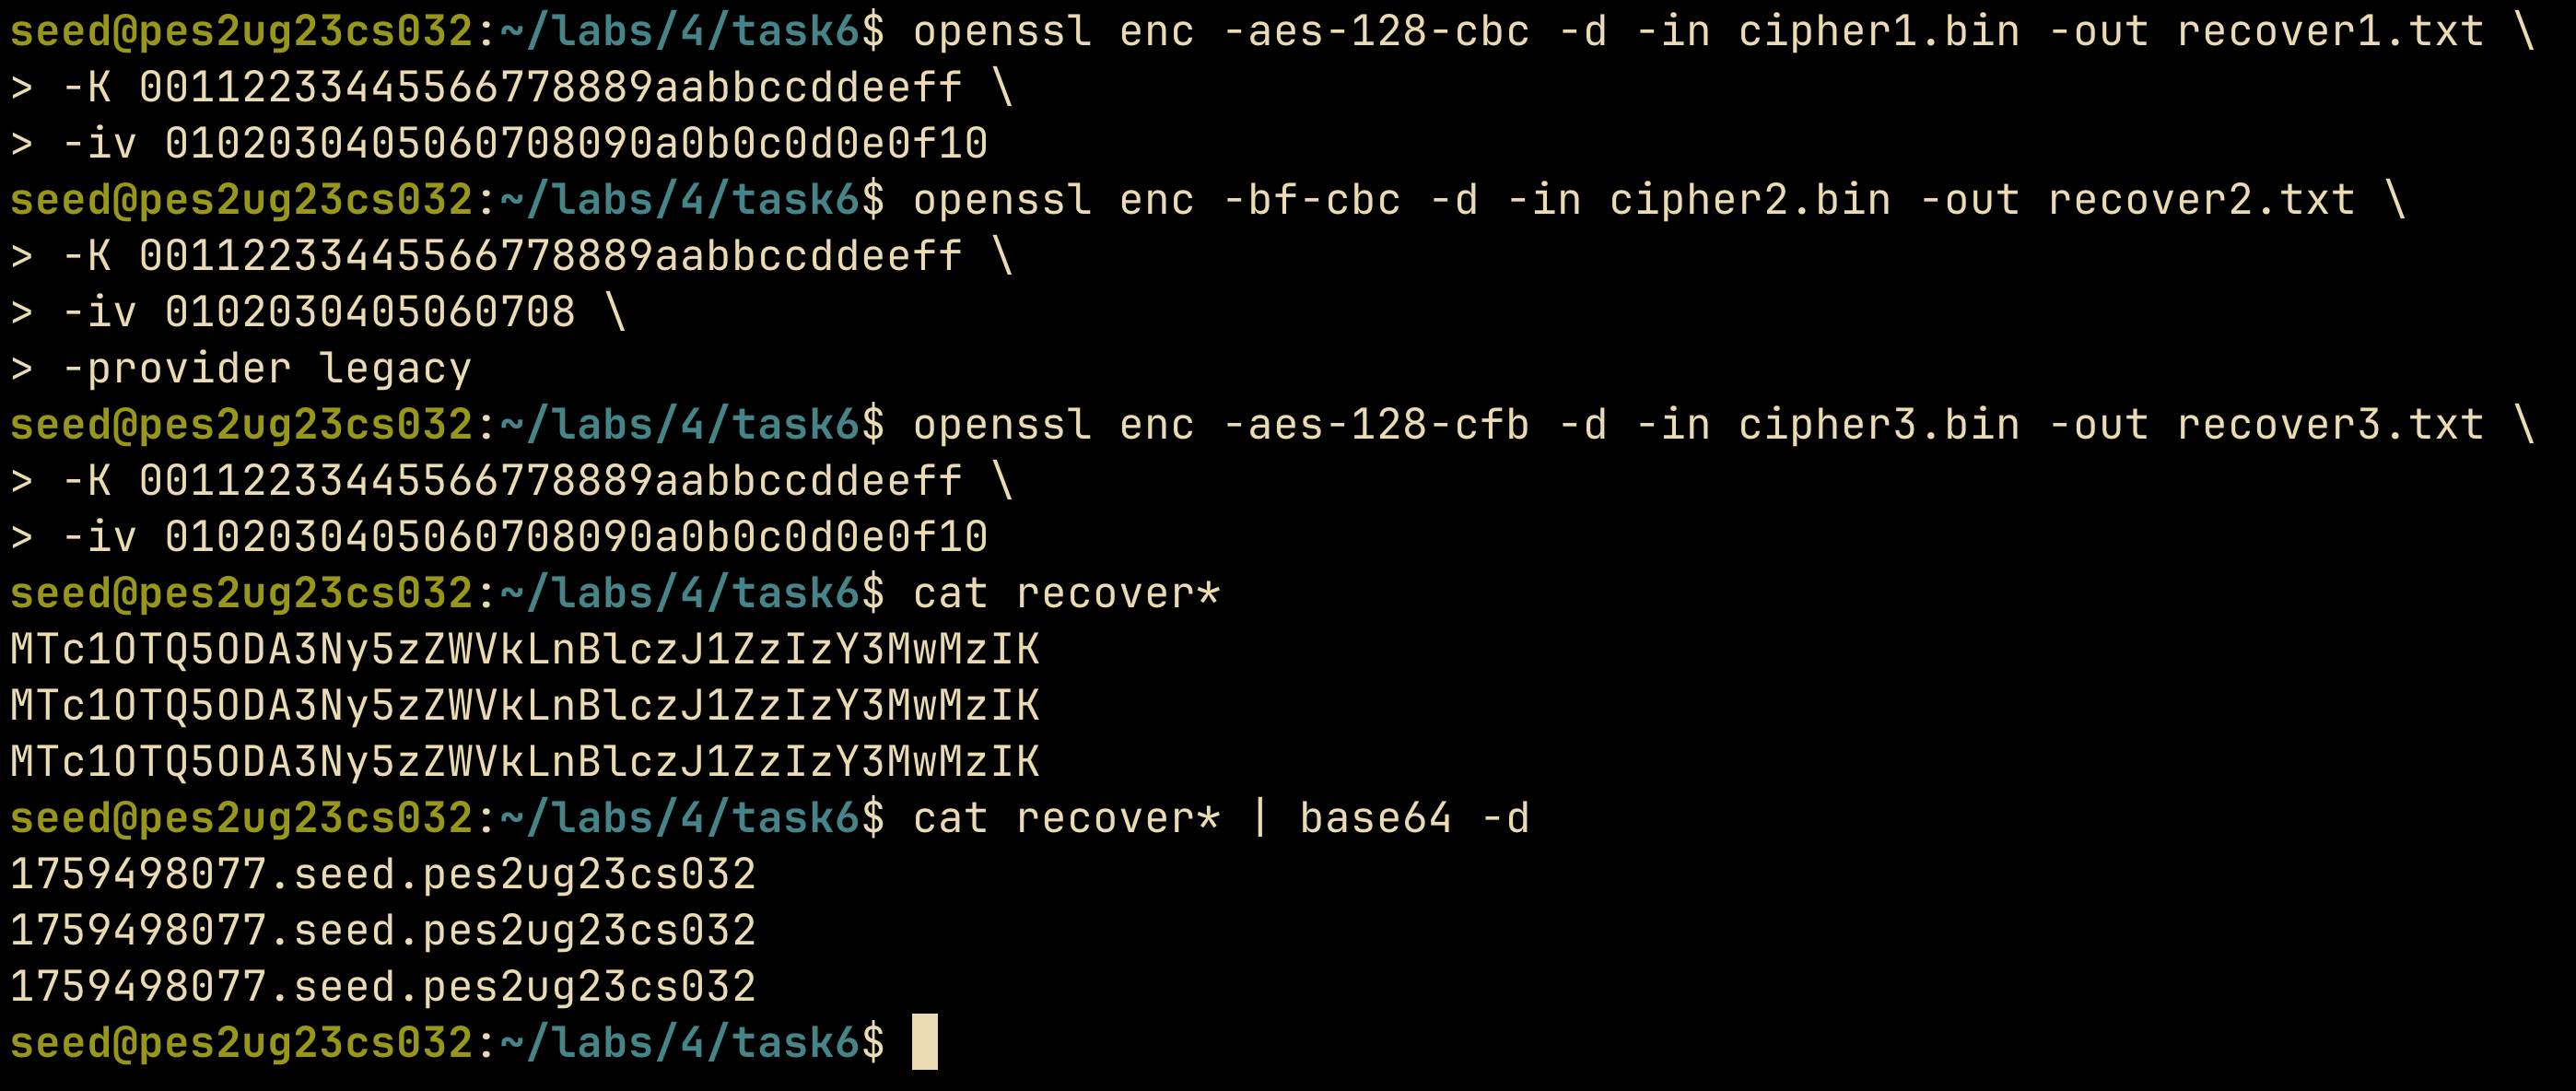
\includegraphics[width=0.8\textwidth]{./images/task6-3.png} 
    \caption{Decrypting and verifying if it matches with the original plaintext}
\end{figure}

The above task shows the difference between the various algorithms (AES-128-CBC mode, Blowfish CBC and AES-128-CFB mode).

\pagebreak

\section{Task 7: Encryption mode - ECB vs CBC}

This tasks focuses on ECB vs CBC on bmp images. Each bmp image has a header of 54 bytes which we do not encrypt, the remaining body of the bmp image is encrypted with AES and concatenated with the header to form a valid bmp image.

\begin{figure}[H]
    \centering
    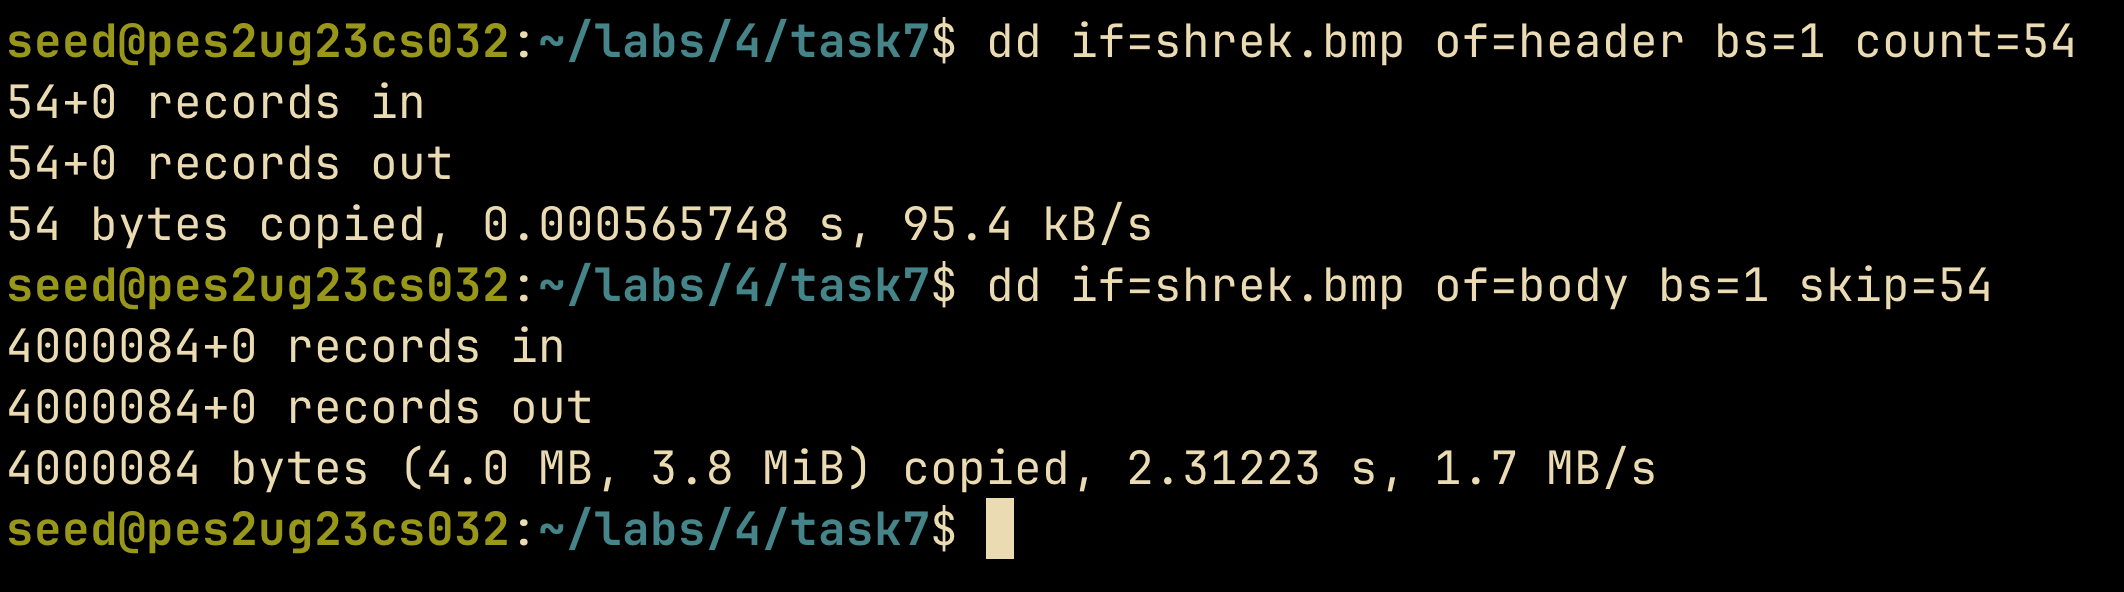
\includegraphics[width=0.8\textwidth]{./images/task7-1.png} 
    \caption{Separating out the header and the body of the bmp image}
\end{figure}

\begin{figure}[H]
    \centering
    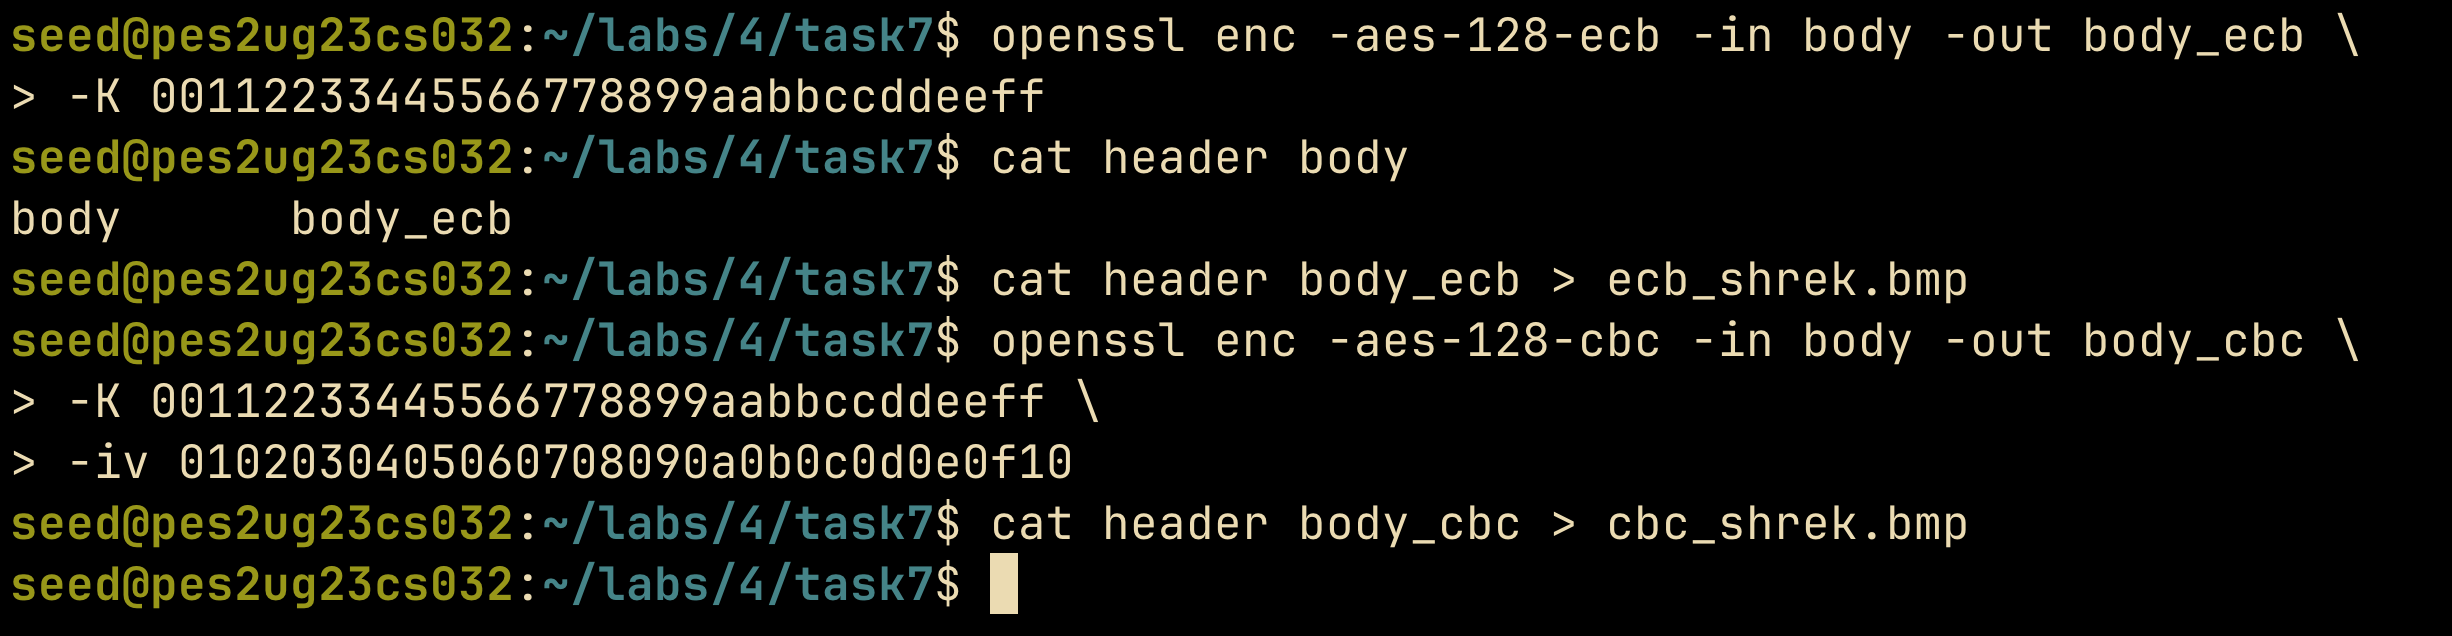
\includegraphics[width=0.8\textwidth]{./images/task7-2.png} 
    \caption{Concatenating header with each encrypted body for ECB and CBC mode}
\end{figure}

\begin{figure}[H]
    \centering
    \includegraphics[width=0.8\textwidth]{./images/task7-3.png} 
    \caption{Comparing CBC(left) and ECB(middle) mode encrypted image with the original(right)}
\end{figure}

The ECB mode still retains some detail of the original image, wheras the CBC mode is not recognizable. This is because identical plaintext blocks produce identical
ciphertext blocks, leaking visual information. CBC mode on the other hand hides repeating patterns by XORing each plaintext block with the previous ciphertext block before encryption, making it more secure for image data.


Decrypting the images back to the original bmp in the same way yields the original image.

\begin{figure}[H]
    \centering
    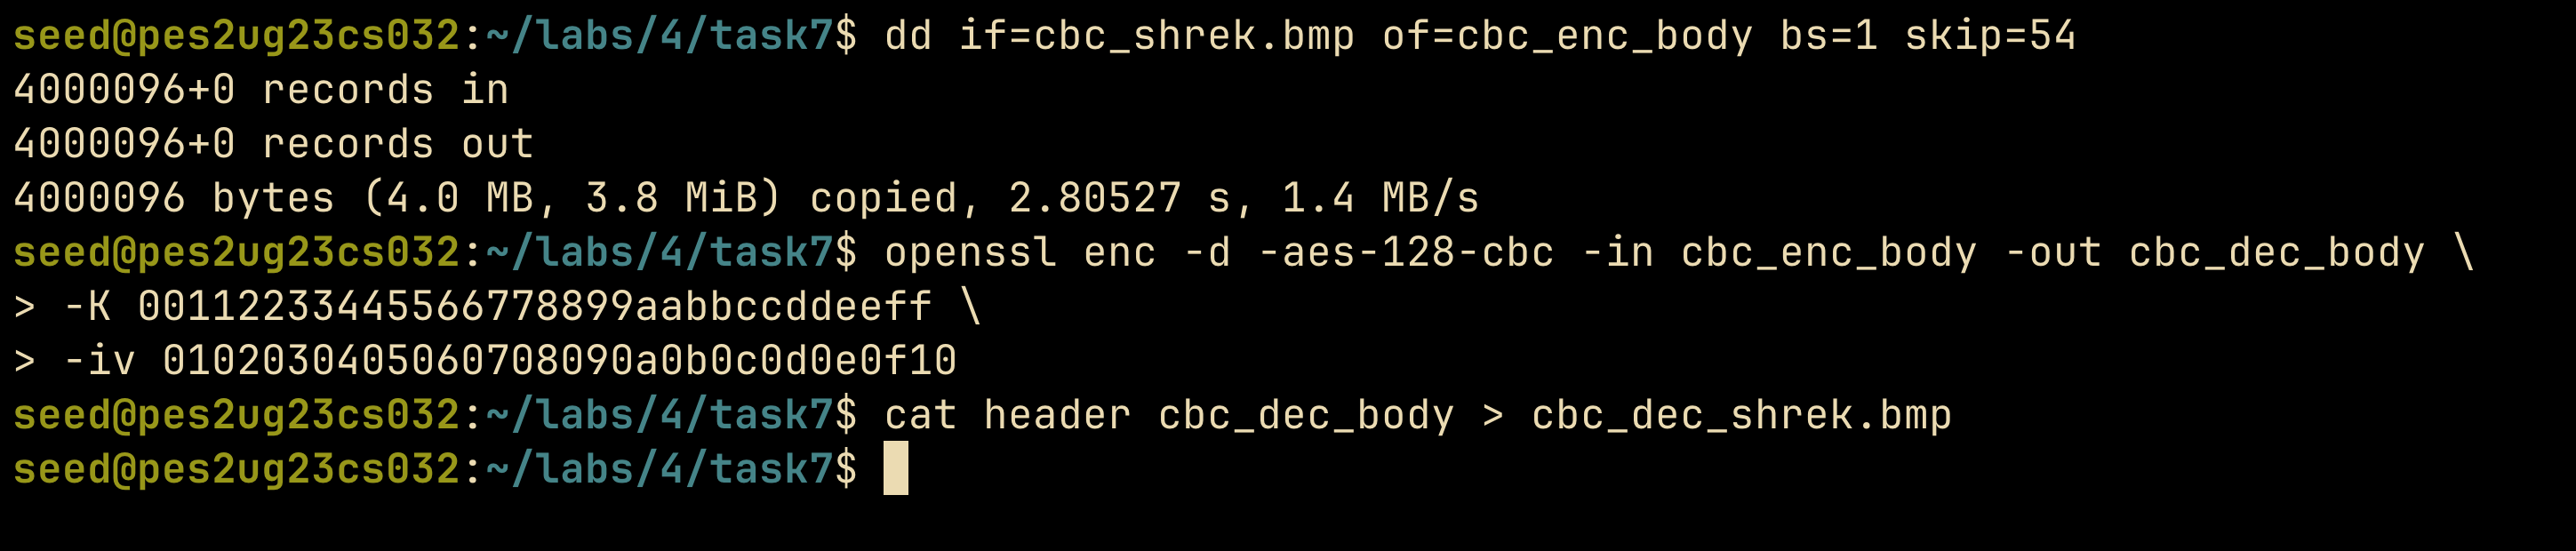
\includegraphics[width=0.8\textwidth]{./images/task7-5.png} 
    \caption{Example of decrypting the CBC encrypted image back to original}
\end{figure}

\begin{figure}[H]
    \centering
    \includegraphics[width=0.8\textwidth]{./images/task7-4.png} 
\end{figure}


\begin{figure}[H]
    \centering
    \includegraphics[width=0.8\textwidth]{./images/task7-6.png} 
\end{figure}

\end{document}